%%%%%%%%%%%%%%%%%%%%%%%%%%%%%%%%%%%%%%%%%12pt: grandezza carattere
                                        %a4paper: formato a4
                                        %openright: apre i capitoli a destra
                                        %twoside: serve per fare un
                                        %   documento fronteretro
                                        %report: stile tesi (oppure book)
\documentclass[12pt,a4paper,openright,twoside]{report}
%
%%%%%%%%%%%%%%%%%%%%%%%%%%%%%%%%%%%%%%%%%libreria per scrivere in italiano
\usepackage[italian]{babel}
%
%%%%%%%%%%%%%%%%%%%%%%%%%%%%%%%%%%%%%%%%%libreria per accettare i caratteri
                                        %   digitati da tastiera come è à
                                        %   si può usare anche
                                        %   \usepackage[T1]{fontenc}
                                        %   però con questa libreria
                                        %   il tempo di compilazione
                                        %   aumenta
\usepackage[utf8]{inputenc}
%
%%%%%%%%%%%%%%%%%%%%%%%%%%%%%%%%%%%%%%%%%libreria per impostare il documento
\usepackage{fancyhdr}
%
%%%%%%%%%%%%%%%%%%%%%%%%%%%%%%%%%%%%%%%%%libreria per avere l'indentazione
%%%%%%%%%%%%%%%%%%%%%%%%%%%%%%%%%%%%%%%%%   all'inizio dei capitoli, ...
\usepackage{indentfirst}
%
%%%%%%%%%libreria per mostrare le etichette
%\usepackage{showkeys}
%
%%%%%%%%%%%%%%%%%%%%%%%%%%%%%%%%%%%%%%%%%libreria per inserire grafici
\usepackage{graphicx}
%
%%%%%%%%%%%%%%%%%%%%%%%%%%%%%%%%%%%%%%%%%libreria per utilizzare font
                                        %   particolari ad esempio
                                        %   \textsc{}
\usepackage{newlfont}
%
%%%%%%%%%%%%%%%%%%%%%%%%%%%%%%%%%%%%%%%%%librerie matematiche
\usepackage{notoccite}
\usepackage{amssymb}
\usepackage{amsmath}
\usepackage{latexsym}
\usepackage{amsthm}
\usepackage{cite}
\usepackage{listings}
\usepackage{hyperref} 
\usepackage[square,numbers,sort]{natbib} 
\usepackage{url}
\usepackage{tabu}
\usepackage{float}
\usepackage{titlesec}

\setcounter{secnumdepth}{4}

\titleformat{\paragraph}
{\normalfont\footnotesize\bfseries}{\theparagraph}{1em}{}
\titlespacing*{\paragraph}
{0pt}{3.25ex plus 1ex minus .2ex}{1.5ex plus .2ex}

\bibliographystyle{unsrt}
%\bibliographystyle{unsrtnat}

\usepackage{listings}
\usepackage{xcolor}
\definecolor{light-gray}{gray}{0.95}
\definecolor{codegreen}{rgb}{0,0.6,0}
\definecolor{codegray}{rgb}{0.5,0.5,0.5}
\definecolor{codepurple}{rgb}{0.58,0,0.82}
\definecolor{backcolour}{rgb}{0.95,0.95,0.92}
\newcommand{\code}[1]{\colorbox{light-gray}{\texttt{#1}}}

\lstdefinestyle{codeblock}{
    backgroundcolor=\color{backcolour},   
    commentstyle=\color{codegreen},
    keywordstyle=\color{magenta},
    numberstyle=\tiny\color{codegray},
    stringstyle=\color{codepurple},
    basicstyle=\ttfamily\footnotesize,
    breakatwhitespace=false,         
    breaklines=true,                 
    captionpos=b,                    
    keepspaces=true,                 
    numbers=left,                    
    numbersep=5pt,                  
    showspaces=false,                
    showstringspaces=false,
    showtabs=false,                  
    tabsize=2
}
 
\lstset{
	style=codeblock,
	frame=single,
	breaklines=true
}


%
\oddsidemargin=30pt \evensidemargin=20pt%impostano i margini
\hyphenation{sil-la-ba-zio-ne pa-ren-te-si}%serve per la sillabazione: tra parentesi 
					   %vanno inserite come nell'esempio le parole 
%					   %che latex non riesce a tagliare nel modo giusto andando a capo.

%
%%%%%%%%%%%%%%%%%%%%%%%%%%%%%%%%%%%%%%%%%comandi per l'impostazione
                                        %   della pagina, vedi il manuale
                                        %   della libreria fancyhdr
                                        %   per ulteriori delucidazioni
\pagestyle{fancy}\addtolength{\headwidth}{20pt}
\renewcommand{\chaptermark}[1]{\markboth{\thechapter.\ #1}{}}
\renewcommand{\sectionmark}[1]{\markright{\thesection \ #1}{}}
\rhead[\fancyplain{}{\bfseries\leftmark}]{\fancyplain{}{\bfseries\thepage}}
\cfoot{}
%%%%%%%%%%%%%%%%%%%%%%%%%%%%%%%%%%%%%%%%%
\linespread{1.3}                        %comando per impostare l'interlinea
%%%%%%%%%%%%%%%%%%%%%%%%%%%%%%%%%%%%%%%%%definisce nuovi comandi
%

%%%%%%%%%%%%%%%%%%%%%%%%%%%%%%%%%%%%%%
% Comandi Custom %
%%%%%%%%%%%%%%%%%%%%%%%%%%%%%%%%%%%%%%
\newcommand{\xsubject}{Web Semantico}
\newcommand{\xstudent}{Andrea Betti}
\newcommand{\xsupervisor}{\\Antonella Carbonaro}



%%%%%%%%%%%%%%%%%%%%%%%%%%%%%%%%%%%%%%
% Fine Preambolo %
% Inizio documento%
%%%%%%%%%%%%%%%%%%%%%%%%%%%%%%%%%%%%%%


\begin{document}

	%%%%%%%%%%%%%%%%%%%%%%%%%%%%%%%%%%%%%%%%
	% Scelta delle dimensioni della pagina %
	%%%%%%%%%%%%%%%%%%%%%%%%%%%%%%%%%%%%%%%%

	%\setlength{\textwidth}{13.5cm}
	%\setlength{\textheight}{19cm}
	%\setlength{\footskip}{3cm}
	
	%%%%%%%%%%%%%%%%%%%%%%%%%
	% inizio prefazione
	%
	% pagina del titolo, indice, sommario
	%%%%%%%%%%%%%%%%%%%%%%%%%
	
	
%\textwidth=450pt
\oddsidemargin=25pt

\begin{titlepage}
\begin{center}
{{\Large{\textsc{Alma Mater Studiorum}}}\\
{\Large{\textsc{Universit\`a di Bologna}}} \\
{\textsc{Campus di Cesena}}} \rule[0.1cm]{14cm}{0.1mm}
		\rule[0.5cm]{14cm}{0.6mm}
{\small{\bf DIPARTIMENTO DI INFORMATICA – SCIENZA E INGEGNERIA\\
Corso di Laurea Magistrale in Ingegneria e Scienze Informatiche }}
\end{center}
\vspace{15mm}
\begin{center}
{\LARGE{\bf Studio e progettazione di tecniche per}}\\
\vspace{2mm}
{\LARGE{\bf l'estrazione automatica di metadati}}\\
\vspace{2mm}
{\LARGE{\bf relativi all'accessibilità delle risorse}}\\
\vspace{2mm}
{\LARGE{\bf didattiche}}\\
\end{center}
\vspace{3mm}
\begin{center}
{Relazione finale in}\\
\vspace{2mm}
{\bf \xsubject}\\
\end{center}
\vspace{20mm}
\par
\noindent
\begin{minipage}[t]{0.5\textwidth}
{\large{\bf Relatore:\\
Prof.ssa \xsupervisor}} \\
\end{minipage}
\hfill
\begin{minipage}[t]{0.47\textwidth}\raggedleft
{\large{\bf Presentata da:\\
\xstudent}}
\end{minipage}
\vspace{30mm}
\begin{center}
{\large{\bf Sessione III\\%inserire il numero della sessione in cui ci si laurea
Anno Accademico 2020-2021}}%inserire l'anno accademico a cui si è iscritti
\end{center}

\newpage
\clearpage{\pagestyle{empty}\cleardoublepage}
\end{titlepage}



	%\begin{titlepage}                       %crea un ambiente libero da vincoli
                                        %   di margini e grandezza caratteri:
                                        %   si pu\`o modificare quello che si
                                        %   vuole, tanto fuori da questo
                                        %   ambiente tutto viene ristabilito
%
\thispagestyle{empty}                   %elimina il numero della pagina
\topmargin=6.5cm                        %imposta il margina superiore a 6.5cm
\raggedleft                             %incolonna la scrittura a destra
\large                                  %aumenta la grandezza del carattere
                                        %   a 14pt
\em                                     %emfatizza (corsivo) il carattere
Questa \`e la \textsc{Dedica}:\\
ognuno pu\`o scrivere quello che vuole, \\
anche nulla \ldots                      %\ldots lascia tre puntini
\newpage                                %va in una pagina nuova

%
%%%%%%%%%%%%%%%%%%%%%%%%%%%%%%%%%%%%%%%%
\clearpage{\pagestyle{empty}\cleardoublepage}%non numera l'ultima pagina sinistra
\end{titlepage}
    
    %
%%%%%%%%%%%%%%%%%%%%%%%%%%%%%%%%%%%%%%%%
\pagenumbering{roman}                   %serve per mettere i numeri romani
\chapter*{Introduzione}                 %crea l'introduzione (un capitolo
                                        %   non numerato)
%%%%%%%%%%%%%%%%%%%%%%%%%%%%%%%%%%%%%%%%%imposta l'intestazione di pagina
\rhead[\fancyplain{}{\bfseries
INTRODUZIONE}]{\fancyplain{}{\bfseries\thepage}}
\lhead[\fancyplain{}{\bfseries\thepage}]{\fancyplain{}{\bfseries
INTRODUZIONE}}
%%%%%%%%%%%%%%%%%%%%%%%%%%%%%%%%%%%%%%%%%aggiunge la voce Introduzione
                                        %   nell'indice
\addcontentsline{toc}{chapter}{Introduzione}

I progressi nelle tecnologie dell'informazione e della comunicazione, e in particolare nell'ingegneria multimediale, di rete e del software, hanno promosso una nuova generazione di ambienti di apprendimento online.

Molte organizzazioni, sia pubbliche che private, sfruttano le nuove tecnologie per offrire prodotti e servizi didattici e formativi a tutti i livelli. In particolare, l'ampia disponibilità di risorse educative è un obiettivo comune per università, biblioteche, archivi e altre istituzioni ad alta intensità di conoscenza.

\vspace{5mm}

Il progetto di tesi vede come oggetto lo sviluppo di un'applicazione web che permetta a studenti universitari di sottoporre le proprie generalità a un sistema di raccomandazione di corsi accademici e relative risorse didattiche associate, dando rilevanza anche alle eventuali disabilità possedute dallo studente.

Il modello di raccomandazione si basa su regole che estendono e inferiscono nuove relazioni semantiche tra i componenti dell'ontologia \textit{Pathadora}, progettata ad-hoc dal collega Sokol Guri per rappresentare i componenti del dominio, incorporando ontologie già esistenti che modellano l'accessibilità delle risorse e l’organizzazione strutturale delle istituzioni educative. 

\vspace{5mm}

L'applicazione permetterà inoltre ai docenti universitari di associare nuove risorse ai corsi di cui sono titolari, su cui verranno generati automaticamente metadati relativi alle proprietà del file e al suo contenuto. Questi metadati verranno utilizzati dal sistema di raccomandazione per suggerire risorse il cui grado di accessibilità secondo determinati aspetti, come la modalità di fruizione del contenuto o la sua trasformabilità, è compatibile con le eventuali disabilità possedute dallo studente.

\vspace{5mm}

Verranno inoltre analizzate varie tecniche di generazione automatica di metadati, il cui scopo è facilitare l'estrazione di informazioni da associare alle risorse.

\vspace{5mm}

La tesi è strutturata in quattro capitoli:
\begin{enumerate}
\item \textbf{Stato dell'arte}, verranno descritte le tematiche principali che interessano i temi dell'estrazione automatica di metadati e l'utilizzo di questi ultimi nel contesto dell'e-learning;
\item \textbf{Contesto del progetto}, viene descritto in cosa consiste il progetto Pathadora e le relative funzionalità;
\item \textbf{Tecnologie}, analizza i linguaggi e le principali tecnologie utilizzate all’interno del progetto;
\item \textbf{Implementazione}, descrive le tecniche di implementazione impiegate nelle diverse parti dell’applicazione.
\end{enumerate}

%%%%%%%%%%%%%%%%%%%%%%%%%%%%%%%%%%%%%%%%%non numera l'ultima pagina sinistra
\clearpage{\pagestyle{empty}\cleardoublepage}

\tableofcontents                        %crea l'indice
%%%%%%%%%%%%%%%%%%%%%%%%%%%%%%%%%%%%%%%%%imposta l'intestazione di pagina
\rhead[\fancyplain{}{\bfseries\leftmark}]{\fancyplain{}{\bfseries\thepage}}
\lhead[\fancyplain{}{\bfseries\thepage}]{\fancyplain{}{\bfseries
INDICE}}
%%%%%%%%%%%%%%%%%%%%%%%%%%%%%%%%%%%%%%%%%non numera l'ultima pagina sinistra
\clearpage{\pagestyle{empty}\cleardoublepage}
\listoffigures                          %crea l'elenco delle figure
%%%%%%%%%%%%%%%%%%%%%%%%%%%%%%%%%%%%%%%%%non numera l'ultima pagina sinistra
\clearpage{\pagestyle{empty}\cleardoublepage}
\listoftables                           %crea l'elenco delle tabelle
%%%%%%%%%%%%%%%%%%%%%%%%%%%%%%%%%%%%%%%%%non numera l'ultima pagina sinistra
    
    

	
	%%%%%%%%%%%%%%%%%%%%%%%%%
	% inizio corpo del documento
	%
	% sequenze delle varie sezioni
	% è consigliato mantenere una struttura logica ben definita per separare le sezioni
	% si consiglia di reificare tale struttura fisicamente sul file system
	%%%%%%%%%%%%%%%%%%%%%%%%%
	

	
	% inclusione delle sezioni
	\clearpage{\pagestyle{empty}\cleardoublepage}
%%%%%%%%%%%%%%%%%%%%%%%%%%%%%%%%%%%%%%%%%imposta l'intestazione di pagina
\lhead[\fancyplain{}{\bfseries\thepage}]{\fancyplain{}{\bfseries\rightmark}}
\pagenumbering{arabic}                  %mette i numeri arabi
\chapter{Stato dell'arte}
\section{Metadati}
I \textit{metadati} sono informazioni associate ad una pagina web o ad una porzione di essa che ne descrivono il contenuto, permettendo che i risultati delle ricerche degli utenti abbiano una maggiore efficacia.

Una volta definiti, i metadati possono essere condivisi e riutilizzati in più occasioni. Questo riutilizzo comporta i seguenti vantaggi:
\begin{itemize}
\item aumentare l'interoperabilità tra diversi sistemi che condividono dati e servizi.
\item ridurre i costi nello sviluppo di sistemi interoperabili, poiché il riutilizzo evita il trattamento delle ambiguità all'interno delle applicazioni.
\item facilitare il trattamento dei dati nei sistemi informativi in genere, ed in particolare in quelli che integrano e condividono dati, ad esempio, sistemi di supporto per il processo decisionale.
\end{itemize}

I metadati possono essere raggruppati o strutturati come “schemi di metadati”, un insieme di metadati progettati per uno scopo specifico, come la descrizione di un tipo di informazioni su una risorsa. La definizione o il significato degli elementi in sé è noto come semantica dello schema. I valori dati agli elementi dei metadati sono il suo contenuto. Gli schemi di metadati di solito specificano i nomi degli elementi e la loro semantica.

Per garantire un alto livello di consistenza dei contenuti, è possibile specificare regole di contenuto, ovvero linee guida che prescrivono quale tipo di informazione è registrata in ogni elemento di metadati, dove trovare le informazioni (es. da un'intestazione di pagina web, una didascalia di una fotografia, ecc.) e come l'informazione è formattata. 

Uno schema di metadati senza regole di sintassi stabilite è chiamato sintassi indipendente.

I metadati possono essere codificati in qualsiasi sintassi definibile come SGML, XML o JSON.

Gli schemi di metadati sviluppati e mantenuti da organizzazioni standard (come ISO) o organizzazioni che hanno assunto tale responsabilità (come la Dublin Core Metadata Initiative) sono chiamati standard di metadati.

I metadati sono generalmente classificati in tre tipi:
\begin{itemize}
\item \textit{metadati descrittivi}, descrivono una risorsa informativa per l'identificazione e il recupero attraverso elementi come titolo, autore e abstract.
\item \textit{metadati strutturali}, documentano le relazioni tra gli oggetti attraverso elementi come i collegamenti ad altri componenti (ad esempio, come le pagine vengono messe insieme per formare i capitoli).
\item \textit{metadati amministrativi}, aiutano a gestire le risorse informative attraverso elementi quali il numero di versione, la data di archiviazione e altre informazioni tecniche ai fini della gestione dei file, della gestione dei diritti e della conservazione.
\end{itemize}

\section{Metodi di generazione automatica di metadati}
Generare metadati di buona qualità in modo efficiente è essenziale per organizzare e rendere accessibile la grande quantità di risorse presente sul web. Il successo di biblioteche digitali, il sostenimento dell'interoperabilità e l'evoluzione del web semantico dipendono da una generazione di metadati efficiente\cite{metadata}.

\vspace{5mm}

L'utilizzo di strumenti automatici di generazione di metadati può facilitare la gestione di una quantità sempre crescente di informazioni.
Idealmente, questi strumenti sono capaci di estrarre informazioni da risorse strutturate e non strutturate, creando metadati di qualità che possano permettere interoperabilità semantica.

\vspace{5mm}

Tra i benefici delle generazione automatica di metadati vi è la scalabilità, per coprire la metadatazione di grandi quantità di informazioni che richiederebbe molto tempo se venisse gestita tutta manualmente, e la consistenza nella generazione dei dati.

A differenza della generazione manuale dei metadati, la generazione automatica dei metadati si basa su metodi automatici per assistere o completare il processo di creazione dei metadati. Greenberg ha distinto due metodi di generazione automatica dei metadati: l'estrazione dei metadati (\textit{metadata extraction}) e la raccolta dei metadati (\textit{metadata harvesting}).
L'estrazione dei metadati utilizza l'indicizzazione automatica e le tecniche di recupero delle informazioni per generare metadati strutturati utilizzando il contenuto originale delle risorse. La raccolta di metadati consiste invece nel raccogliere in modo automatico metadati già prodotti e archiviati da diversi repository.

\vspace{5mm}

All'interno di questa dicotomia di metodi di estrazione, vi sono molte tecniche più specifiche che i ricercatori hanno sviluppato per la generazione automatica di metadati. Polfreman et al. ha identificato sei tecniche che sono state sviluppate nel corso degli anni: \textit{raccolta di meta-tag}, \textit{estrazione di contenuti}, \textit{indicizzazione automatica}, \textit{text e data mining}, \textit{autogenerazione di dati estrinseci} e \textit{social tagging}. Sebbene l'ultima tecnica non sia propriamente una tecnica di generazione automatica di metadati, poiché viene utilizzata per generare metadati con un intervento minimo richiesto dai professionisti dei metadati, può essere vista come una possibile modalità per semplificare il processo di creazione dei metadati\cite{semi}.

\subsection{Estrazione di meta-tag}
L'\textbf{estrazione di meta-tag} è un processo dove vengono identificati valori per campi di metadati e popolati attraverso l'osservazione dei tag associati ai documenti, di fatto convertendo i metadati raccolti da più repository in formati diversi.

La più grande debolezza di questo tipo di tool è il fatto che la sua efficacia dipenda dalla qualità dei metadati raccolti.
Tra i tool che sfruttano questa tecnica vi sono MarcEdit, che mediante appositi harvester raccoglie metadati da record conformi al protocollo \textbf{Open Archives Initiative Protocol for Metadata Harvesting} (\textbf{OAI-PMH}) e che può convertire in diversi formati (MARC, MARC XML, MODS, EAD), e tool come Editor-Converter Dublin Core Metadata e Firefox Dublin Core Viewer Extension che convertono informazioni trovate nei meta-tags dei file HTML trovati sul web in elementi Dublin Core.

L'OAI-PMH fornisce un framework di interoperabilità, indipendente dall'applicazione, basata sul raccoglimento dei metadati. Il framework di OAI-PMH comprende i service provider, che eseguono richieste per effettuare la raccolta dei metadati, e i data provider, che espongono i metadati. OAI-PMH è largamente utilizzato da biblioteche digitali, repository istituzionali e archivi digitali\cite{harvesting}. Alcuni esempi di archivi che implementano OAI-PMH sono:

\begin{itemize}
\item Digital Public Library of America (DPLA), aggrega metadati relativi a enti istituzionali americani
\item National Science Digital Library (NSDL), è un libreria digitale ad accesso libero contenente collezioni di metadati inerenti a scienze, tecnologia, ingegneria e matematica
\item OAIster, un catalogo di milioni di record relativi a risorse di fonti eterogenee
\item Open Language Archives Community (OLAC), una libreria virtuale di risorse linguistiche
\end{itemize}

\subsection{Estrazione di contenuti}
L'\textbf{estrazione di contenuti} è una forma di estrazione di metadati che sfrutta algoritmi di machine learning per associare parole chiave al documento sulla base del suo contenuto. Il vantaggio di questo approccio è che il risultato è indipendente dalla qualità dei metadati associati alla risorsa. Esempi di applicazioni che impiegano questa tecnica sono Kea, che utilizza le tecniche TF-IDF e first-occurence per identificare e assegnare frasi chiave da risorse testuali, e Open Text Summarizer che esegue l'estrazione automatica di un riassunto del testo passato in input e delle relative parole chiave. 

I metodi di estrazione di parole chiave possono essere suddivisi in tre categorie: metodi statistici, metodi basati sui grafi e metodi basati sul deep learning\cite{extraction}.

\subsubsection{Metodi statistici}
I \textbf{metodi statistici} sono i più semplici. Calcolano le statistiche per le parole chiave e utilizzano tali statistiche per valutarle. Tra questi metodi rientrano il calcolo la frequenza delle parole, la collocazione linguistica, la co-occorrenza e tecniche più sofisticate come TF-IDF e YAKE!.

\textbf{TF-IDF} (Term Frequency–Inverse Document Frequency) stima l'importanza della parola nel documento rispetto all'intero corpus (insieme di più documenti). Calcola la frequenza di ogni termine nel documento e la pondera con l'inverso della frequenza del termine nell'intero corpus. Le parole chiave verranno selezionate tra i termini con i punteggi più alti. Questo algoritmo favorisce i termini frequenti nel documento di testo e non frequenti negli altri documenti. Il vantaggio di TF-IDF è che è veloce e lo svantaggio è che necessita di un corpus di almeno qualche dozzina di documenti. TF-IDF è indipendente dalla lingua.

\textbf{YAKE!} (Yet Another Keyword Extractor) è un metodo di estrazione di parole chiave che utilizza feature statistiche ricavate da un singolo documento per estrarre le parole chiave. Estrae le parole chiave in cinque passaggi:
\begin{enumerate}
\item \textbf{Pre-elaborazione e identificazione del termine candidato}: il testo è suddiviso in frasi, blocchi (parte della frase separata da punteggiatura) e token. Il testo viene pulito, etichettato e vengono identificate le stop words.
\item \textbf{Estrazione delle caratteristiche}: calcola le seguenti cinque feature statistiche per i termini (parole) nel documento:
\begin{itemize}
\item Casing: conta il numero di volte (in proporzionale al numero complessivo di volte in cui compare) in cui il termine appare in maiuscolo o come acronimo nel testo. Un termine significativo di solito appare più spesso in maiuscolo.
\item Posizione del termine: posizione mediana della frase del termine nel testo. I termini più vicini all'inizio tendono a essere i più significativi.
\item Normalizzazione della frequenza dei termini: misura la frequenza bilanciata dei termini nel documento.
\item Relazione del termine al contesto: misura con quanti termini diversi il termine candidato coesiste. Termini più significativi coesistono con meno termini diversi. 
\item Termine in frasi diverse: misura quante volte i termini compaiono in frasi diverse. Un punteggio più alto indica un termine più significativo.
\end{itemize}
\item \textbf{Calcolo del punteggio del termine}: le funzioni del passaggio precedente vengono combinate in un unico punteggio.
\item \textbf{Generazione di n-grammi e calcolo dei punteggi delle parole chiave}: l'algoritmo identifica tutti gli n-grammi validi. Le parole negli n-grammi devono appartenere allo stesso blocco e non devono iniziare o terminare con una stopword. Successivamente, ogni n-gramma viene valutato moltiplicando i punteggi dei suoi membri e normalizzato per ridurre l'impatto della lunghezza dell'n-gramma. Le stopword vengono trattate in modo diverso per ridurre al minimo il loro impatto.
\item \textbf{Deduplicazione e ranking dei dati}: vengono rimosse le parole chiavi simili tra loro.
\end{enumerate}

\subsubsection{Metodi basati sui grafi}
I metodi basati su grafi generano un grafo dei termini correlati presenti nei documenti. Un grafo, ad esempio, può collegare i termini che si verificano contemporaneamente nel testo. I metodi basati su grafi utilizzano metodi di classificazione che considerano la struttura del grafo per valutare l'importanza del vertice. Uno dei metodi di questa categoria più conosciuti è TextRank.

\textbf{TextRank} è un metodo di classificazione basato su grafi utilizzato per estrarre frasi pertinenti o trovare parole chiave. L'estrazione delle parole chiave avviene in cinque passaggi:

\begin{itemize}
\item \textbf{Tokenizzazione e annotazione del testo} con tag di Part of Speech (PoS) (nomi, articoli, verbi...)
\item \textbf{Costruzione del grafo di co-occorrenza di parole}: i vertici nel grafo sono parole con tag PoS selezionati. Due vertici sono collegati con un arco se compaiono all'interno della finestra di N parole nel testo. Il grafo è non orientato e non ponderato.
\item \textbf{Graph ranking}: partendo con il punteggio di ciascun vertice inizializzato a 1, viene applicato sul grafo l'algoritmo di ranking utilizzando la seguente equazione:
\begin{equation}
S(Vi)=(1 - d) + d\left (\sum_{j \in In(Vi)} \frac{S(Vj)}{|Out(Vj)|}\right )
\end{equation}
Il peso \textit{S(Vi)} di un vertice \textit{Vi} è calcolato considerando i pesi dei vertici connessi al nodo \textit{Vi}. Nell'equazione, \textit{d} è il fattore di smorzamento impostato su 0,85. Gli \textit{In(Vi)} corrispondono ai collegamenti in entrata al vertice \textit{Vi} e gli \textit{Out(Vj)} ai collegamenti in uscita dal vertice \textit{Vj}. Poiché stiamo considerando grafi non orientati, un collegamento in entrata verso un nodo è anche un collegamento in uscita dallo stesso nodo. L'algoritmo viene eseguito su ciascun nodo in diverse iterazioni fino a quando i pesi sui nodi convergono: la variazione tra le iterazioni è inferiore a 0,0001.
\item \textbf{Selezione delle parole con il punteggio più alto}: le parole (quindi i vertici) sono ordinate per punteggio, dal più alto al più basso. Viene poi selezionato il primo terzo delle parole.
\item \textbf{Estrazione delle parole chiave}: in questo passaggio, le parole selezionate nella fase precedente vengono unite in parole chiave composte da più parole se compaiono in una stessa frase. Il punteggio delle parole composte corrisponde alla somma dei punteggi delle parole singole che le compongono.
\end{itemize}

L'algoritmo viene eseguito su ciascun documento separatamente e non necessita di un corpus di documenti per eseguire l'estrazione delle parole chiave. TextRank è indipendente dalla lingua.

\textbf{RAKE} (Rapid Automatic Keyword Extraction) è un altro algoritmo di estrazione delle parole chiave basato su grafi. L'algoritmo si basa sull'osservazione che le parole chiave sono spesso composte da più parole e di solito non includono stop-word o punteggiatura.

Include i seguenti passaggi:
\begin{itemize}
\item \textbf{Estrazione delle parole chiave candidate}: il testo viene suddiviso in base alle parole chiave candidate in base alle parole di arresto e al delimitatore di frase. Una parola chiave candidata è una frase che si trova tra due stop-word o delimitatori di frase. I delimitatori di frase sono, ad esempio, i caratteri di punteggiatura.
\item \textbf{Costruzione del grafo di co-occorrenza delle parole chiave}: i vertici nel grafo corrispondono a parole. Sono collegati se compaiono insieme nelle parole chiave candidate. Il grafo è ponderato: il peso corrisponde al numero di volte in cui le parole collegate appaiono insieme nelle parole chiave candidate. Un vertice può essere collegato a sé stesso nel caso corrisponda a una parola che appare in una parola chiave candidata insieme a sé stessa.
\item \textbf{Punteggio delle parole}: ogni parola nel grafo è valutata con uno dei seguenti punteggi: 
\begin{itemize}
\item \textit{Grado della parola} (\texttt{deg(w)}): numero di parole con cui la parola w co-occorre (somma dei pesi degli archi). Il grado favorisce le parole che compaiono più spesso e in parole chiave più lunghe.
\item \textit{Frequenza della parola} (\texttt{freq(w)}): numero di volte che la parola appare in qualsiasi parola chiave candidata. Questo criterio favorisce le parole che appaiono più frequentemente.
\item \textit{Rapporto tra grado e frequenza} (\texttt{deg(w)/freq(w)}): favorisce le parole che ricorrono principalmente nelle parole chiave candidate più lunghe. Il grado favorirà le parole chiave più brevi.
\end{itemize}
\item \textbf{Punteggio delle parole chiave candidate}: il punteggio di ciascuna parola chiave candidata è la somma dei punteggi delle parole che la compongono.
\item \textbf{Parole chiave adiacenti}: le parole chiave candidate non includono stopword. Poiché a volte le stopword possono essere parte della parola chiave, vengono aggiunte in questo passaggio. L'algoritmo individua le coppie di parole chiave di cui fa parte almeno una stopword e, nel caso quest'ultima sia presente almeno due volte nel testo, le aggiunge all'insieme delle stopword esistenti. Il punteggio della nuova parola chiave è la somma dei punteggi delle parole chiave che la compongono.
\item \textbf{Estrazione delle parole chiave}: viene infine estratto il terzo delle parole chiave con il punteggio migliore.
\end{itemize}

La differenza principale tra RAKE e TextRank è che RAKE considera le ricorrenze all'interno delle parole chiave candidate invece di una finestra fissa. Utilizza una procedura di punteggio più semplice e statistica: non include l'ottimizzazione. L'algoritmo viene eseguito su ciascun documento separatamente, quindi non necessita di un corpus di documenti.

\subsubsection{Metodi basati sul deep learning}
Il deep learning è un’area del machine learning che si basa sull’apprendimento dei dati "in profondità" su più livelli. È caratterizzato dalla creazione di un modello di apprendimento automatico a più strati, nel quale i livelli più profondi prendono in input le uscite dei livelli precedenti, trasformandoli e astraendoli sempre di più.

La comparsa del deep learning ha consentito metodi basati sull'embedding, un insieme di tecniche di modellazione in cui le parole vengono mappate in vettori di numeri reali. 

Questi metodi trovano principalmente un elenco di parole chiave candidate (ad esempio, Bennani et al. considerano solo parole chiave costituite da nomi e aggettivi). Incorporano il documento e le parole chiave candidate nello stesso spazio di inclusione e misurano la similarità (ad es. similarità del coseno) tra i valori del documento e delle parole chiave. Selezionano le parole chiave più simili al testo del documento in base alla misura di similarità.

\subsection{Indicizzazione automatica}
Così come la content extraction, l'\textbf{indicizzazione automatica} prevede l'utilizzo di machine learning e algoritmi rule-based per estrarre metadati dalle risorse. La differenza sta nel fatto che i termini estratti vengono successivamente mappati in vocabolari controllati come Library of Congress Subject Headings (LCSH), Getty Thesaurus of Geographic Names (TGN), Library of Congress Name Authority (LCNA) o ontologie relative a un dominio specifico. I termini determineranno possibili punti di accesso sotto i quali i documenti associati possono essere cercati e identificati.

Il processo di indicizzazione si compone di tre fasi:
\begin{itemize}
\item analisi del documento e individuazione del suo tema di base (il contenuto concettuale).
\item identificazione dei concetti principali presenti in tale contenuto (l'insieme di tali concetti costituisce il "soggetto" del documento stesso).
\item traduzione nei termini di un linguaggio di indicizzazione, utilizzando termini estratti dal documento stesso (indicizzazione derivata, o estratta) oppure avvalendosi di un dizionario controllato ("indicizzazione assegnata")
\end{itemize}

\subsection{Text e data mining}
A causa della complessità delle tecniche utilizzate per l'estrazione di metadati, la maggior parte degli usi di queste tecniche sono stati sviluppati per risolvere i problemi della generazione automatica di metadati nel contesto di specifici progetti di ricerca.
I principali motivi sono il fatto che l'efficacia di queste tecniche dipende dalla qualità e dalla quantità dei dati di training, e che i vocabolari controllati come LCSH sono troppo complicati e diversificati per essere applicati con mezzi automatici.

Il \textbf{text mining} è un campo interdisciplinare che attinge al recupero delle informazioni, al \textbf{data mining}, all'apprendimento automatico, alle statistiche e alla linguistica computazionale. Una parte sostanziale delle informazioni viene memorizzata come testo come articoli di notizie, documenti tecnici, libri, biblioteche digitali, messaggi di posta elettronica, blog e pagine web. Quindi, la ricerca nel text mining è stata molto attiva. Un obiettivo importante è ricavare informazioni di alta qualità dal testo, ovvero rilevanti e di interesse. Ciò avviene in genere attraverso la scoperta di modelli e tendenze mediante l'apprendimento di modelli statistici, la modellazione di argomenti e la modellazione statistica del linguaggio. Solitamente, il text mining richiede la strutturazione del testo di input (ad esempio, l'analisi, l'aggiunta di alcune caratteristiche linguistiche derivate e la rimozione di altre e il successivo inserimento in un database). Questo è seguito dalla derivazione dei modelli all'interno dei dati strutturati e dalla valutazione e interpretazione dell'output.

Le tipiche attività di text mining includono la categorizzazione del testo, il clustering del testo, l'estrazione di concetti/entità, la produzione di tassonomie granulari, l'analisi del sentiment, il riepilogo dei documenti e la modellazione delle relazioni tra entità (ovvero, relazioni di apprendimento tra entità nominate). Altri esempi includono il data mining multilingue, l'analisi del testo multidimensionale, il text mining contestuale e l'analisi della fiducia e dell'evoluzione nei dati di testo, nonché le applicazioni di text mining in materia di sicurezza, analisi della letteratura biomedica, analisi dei media online e gestione analitica delle relazioni con i clienti. Vari tipi di software e strumenti di analisi e estrazione di testo sono disponibili nelle istituzioni accademiche, nei forum open source e nell'industria. L'estrazione di testo utilizza spesso anche WordNet, Sematic Web, Wikipedia e altre fonti di informazioni per migliorare la comprensione e l'estrazione dei dati di testo.\cite{textmining}

\subsection{Autogenerazione di dati estrinseci}
La generazione automatica di dati estrinseci è il processo di estrazione dei metadati su una risorsa informativa che non è contenuta all'interno della risorsa stessa. La generazione automatica di dati estrinseci può includere l'estrazione di metadati tecnici come il formato e le dimensioni del file, ma può essere anche l'estrazione di funzionalità più complesse come il livello di classe scolastica a cui è destinata una risorsa didattica o il tipo di lettori per cui è destinato un documento.
Processi di questo tipo sono difficili da implementare a causa dell'assenza di informazioni sul contesto di una risorsa
contenute nella risorsa stessa.
Tra i tool che implementano questa tecnica di estrazione di metadati vi sono Dspace e JHove.

\subsection{Social Tagging}
Il social tagging è una forma di generazione di metadati, sebbene non propriamente automatica, che permette agli utenti di creare e assegnare tag alle risorse di un sito web. A causa del costo relativamente basso della generazione e del mantenimento dei metadati attraverso il social tagging e della sua attuale popolarità diffusa, alcuni progetti hanno tentato di utilizzare questi dati per migliorare i repository di archiviazione di metadati. Ad esempio, Linstaedt et al. usa programmi per analizzare le immagini statiche trovate all'interno di Flickr e utilizzare questi risultati d'analisi per propagare tag utente pertinenti a nuove immagini elaborate.

Un esempio di utilizzo del social tagging più complesso può consistere nell'utilizzare tecniche di apprendimento automatico, tenendo traccia dei cambiamenti applicati sui metadati associati a una risorsa da parte degli utenti e migliorare quindi i meccanismi di learning del database sulla base di queste modifiche.
Tra i tool che supportano il social tagging vi sono Dspace e Omeka.

Sebbene gli strumenti di generazione automatica di metadati offrano molti vantaggi, soprattutto per quanto riguarda la semplificazione del processo di creazione dei metadati, esistono barriere significative all'adozione e all'implementazione diffusa di questi strumenti. Un problema incontrato con gli strumenti di generazione automatica di metadati è che molti di essi sono sviluppati localmente per soddisfare le esigenze specifiche di un determinato progetto o come parte della ricerca accademica.

Diversi tool sono focalizzati alla risoluzione di pochi problemi specifici legati alla generazione di metadati, come possono essere l'estrazione di parole chiave di Kea piuttosto che l'estrazione di tag HTML e la successiva conversione in elementi Dublin Core di Editor Converter Dublin Core, portando quindi a sforzi significativi per coordinare le applicazioni selezionate e ottenere l'output desiderato.
È inoltre necessaria una buona conoscenza tecnica di linguaggi di programmazione per implementare questi sistemi propriamente.

Un altro problema è la discontinuità delle applicazioni, che possono presto risultare obsolete e perdere supporto tecnico.

\section{Ricerca sul tema}
Gli sforzi di ricerca per la generazione automatica di metadati possono essere classificati in due aree: \textbf{ricerca sperimentale}, focalizzata sulle tecniche di recupero delle informazioni e sui contenuti delle risorse digitali, e \textbf{ricerca applicativa}, riguardante lo sviluppo di software per la creazione di contenuti e strumenti di generazione di metadati utilizzati nel contesto operativo\cite{amega}.

\subsection{Ricerca sperimentale}
La crescita dei repository di risorse digitali fornisce una grande quantità di collezioni per lo studio della generazione automatica di metadati.

I ricercatori che gestiscono il contenuto delle risorse digitali per la generazione di metadati hanno sperimentato principalmente con la \textbf{struttura dei documenti} e i \textbf{sistemi di rappresentazione della conoscenza}.

\subsubsection{Struttura del documento}
I ricercatori hanno identificato relazioni tra genere, contenuto e struttura del documento. Ad esempio, il genere del documento può dare informazioni sulla densità testuale, che può essere utilizzata per prevedere le prestazioni dell'algoritmo di estrazione dei metadati per determinati tipi di documenti.

Il genere del documento inoltre determina una struttura prevedibile che facilita l'estrazione automatica di metadati. Ad esempio, i documenti di ricerca includono informazioni standard come "titolo", "autore" e "affiliazione dell'autore del documento. Gli esperimenti che sfruttano la struttura del documento in questa seconda sede utilizzando un algoritmo Support Vector Machine (SVM) (ad esempio, Han et al., 2003) e Variable Hidden Markov Model (DVHMM) (Takasu, 2003) hanno avuto un discreto successo per la generazione di metadati.

\subsubsection{Sistemi di rappresentazione della conoscenza}
La memorizzazione di metadati può essere eseguita attraverso l'utilizzo di ontologie, thesauri, sistemi classificatori, file di autorità e altri strumenti di rappresentazione della conoscenza.
Attraverso l'utilizzo di regole di inferenza, è possibile generare ulteriori informazioni relative a un oggetto sulla base dei valori delle sue proprietà.

\subsection{Ricerca applicativa}
Tra gli strumenti in grado di generare automaticamente metadati è possibile distinguere i software per la creazione di contenuti da tool più specializzati conosciuti come applicazioni per la generazione di metadati.

\subsubsection{Software per la creazione di contenuti}
Esempi di software per la creazione di contenuti sono Microsoft Word, Adobe Acrobat e Nullsoft Winamp, essenzialmente qualsiasi software che può essere utilizzato per creare contenuti digitali, testuali o multimediali. Nel contesto del web, il software per la creazione di contenuti viene utilizzato per creare una risorsa digitale a cui è possibile accedere tramite un browser e il software associato. Anche un surrogato bibliografico può essere considerato contenuto.

I software per la creazione di contenuti possono supportare la generazione di metadati tramite mezzi automatici, semiautomatici e umani. Le tecniche automatiche sono spesso impiegate per produrre metadati tecnici come la data di creazione, la data dell'ultima modifica, la dimensione in byte e il formato del file.

Alcuni software per la creazione di contenuti estraggono i metadati dal contenuto del documento nel tentativo di fornire rappresentazioni descrittive (ad esempio, Word assegna automaticamente un titolo in base alla prima riga di un documento). Alcuni software per la creazione di contenuti includono un modello per facilitare l'immissione di metadati umani. Le tecniche automatiche possono quindi essere impiegate dall'applicazione per convertire i metadati immessi in un linguaggio di codifica specificato, incorporarli in un'intestazione di risorsa o inserirli in un database di metadati.

\subsubsection{Applicazioni e generazione automatica di metadati}
Le applicazioni per la generazione di metadati differiscono dal software per la creazione di contenuti in quanto sono progettate specificamente e solo per produrre record di metadati. 
La quantità di elaborazione automatica e umana richiesta per produrre metadati distingue i generatori, applicazioni che si basano principalmente su tecniche automatiche, dagli editor, che integrano l'elaborazione automatica con quella umana.

\paragraph{Data Fountains}
Data Fountains è uno strumento utilizzabile non solo per descrivere le risorse Internet, ma in primo luogo per scoprirle. Ha tre funzionalità principali:

\begin{itemize}
\item generazione di metadati per una determinata pagina web dato il suo URL
\item generazione di metadati per le risorse inerenti a un argomenti particolare
\item esecuzione del drill-down dei collegamenti a partire da un URL iniziale al fine di generare record di metadati ed estrarre le parti significative del testo analizzato
\end{itemize}

\paragraph{JHOVE}
\textbf{JHOVE} (JSTOR/Harvard Object Validation Environment) è un framework utilizzabile per eseguire l'identificazione del formato, la validazione e la caratterizzazione di oggetti digitali:

\begin{itemize}
\item L'identificazione del formato è il processo atto a determinare il formato a cui è conforme un oggetto digitale
\item La convalida del formato è il processo di determinazione del livello di conformità di un oggetto digitale alla specifica per il suo presunto formato
\item La caratterizzazione del formato è il processo di determinazione delle proprietà significative specifiche del formato di un oggetto
\end{itemize}

Queste azioni sono spesso necessarie durante il funzionamento di routine degli archivi digitali e per le attività di conservazione digitale.

JHOVE utilizza un'architettura plug-in estensibile; può essere configurato al momento della sua chiamata per includere qualsiasi modulo di formato specifico e gestori di output desiderati. La versione iniziale di JHOVE include moduli per flussi di byte arbitrari, testo codificato ASCII e UTF-8, audio AIFF e WAV, GIF, JPEG, JPEG 2000, TIFF e PDF; e gestori di output di testo e XML.

\paragraph{Kea}
\textbf{Kea} estrae dai documenti testuali n-grammi con lunghezza predefinita che non iniziano o terminano con una stop word. Nell'indicizzazione controllata, raccoglie solo gli n-grammi che corrispondono ai termini presenti nel thesaurus (dizionario dei sinonimi). Se il thesaurus definisce relazioni tra termini non consentiti (non descrittori) e termini consentiti (descrittori), sostituisce ciascun descrittore con un non descrittore equivalente. Per ciascuna frase candidata, Kea computa quattro feature:
\begin{itemize}
\item{\textbf{TF-IDF}}, misura l'importanza di un termine rispetto a una collezione di documenti. Aumenta al numero di volte che il termine è contenuto nel documento, e diminuisce con la frequenza del termine nella collezione proporzionalmente
\item{\textbf{First occurrence}}, è computata come la percentuale della quantità di testo che precede la prima occorrenza del termine nel documento. La probabilità che i termini che compaiono all'inizio dei documenti siano elementi chiave è maggiore rispetto a quella degli altri
\item{\textbf{Lunghezza della locuzione}}, è il numero delle parole che la compongono
\item{\textbf{Grado del nodo}}, è il numero di frasi nel set candidato collegati semanticamente a una specifica frase candidata. A un grado del nodo alto aumenta la probabilità che sia una espressione chiave.
\end{itemize}

Prima di poter estrarre frasi chiave da nuovi documenti, Kea deve prima creare un modello che apprenda la strategia di estrazione dai documenti indicizzati manualmente. Ciò significa che per ciascun documento nella directory di input deve essere presente un file con estensione ".key" e lo stesso nome del documento corrispondente. Questo file dovrebbe contenere frasi chiave assegnate manualmente, una per riga.
Dato l'elenco delle frasi candidate, Kea contrassegna quelle che sono state assegnate manualmente come esempi positivo e tutte le altre come esempi negativi. Analizzando i valori delle feature per le frasi candidate positive e negative, viene calcolato un modello che riflette la distribuzione dei valori delle feature per ciascuna frase.

Una volta terminata la sessione di training, Kea utilizza il modello per calcolare per ogni frase candidata la probabilità di essere una frase chiave considerando le feature calcolate. Le frasi con le probabilità più alte vengono selezionate nella serie finale di frasi chiave. L'utente può specificare il numero di frasi chiave che devono essere selezionate\cite{kea}.

\begin{figure}[H]
\centering
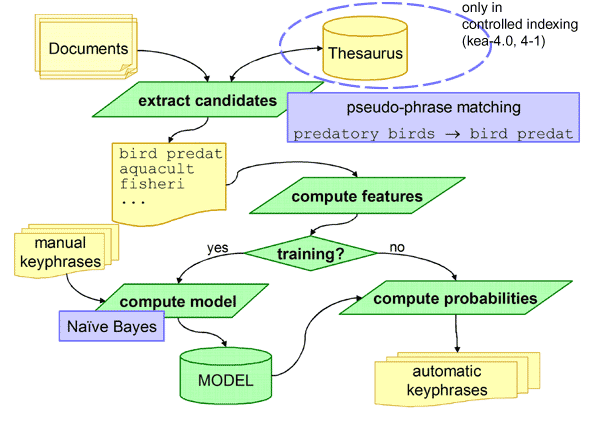
\includegraphics[scale=1]{res/kea_diagram.png}
\caption{Schema di Kea}
\label{fig:kea}
\end{figure}

\subsection{Estrazione del testo da risorse multimediali}
Di seguito viene descritto un possibile approccio per estrarre automaticamente il testo da un file multimediale al fine di analizzarlo con le tecniche viste in precedenza\cite{video}:
\begin{enumerate}
\item \textit{Estrazione audio}: nel caso di un file video, viene eseguita una conversione di formato tra MPEG e WAV tramite uno strumento di conversione per separare l'audio dal video;
\item \textit{Suddivisione dell'audio}: il file WAV viene suddiviso in frammenti da 1 a 2 minuti, in base alla dimensione del file risultante, per evitare un carico computazionale eccessivo;
\item \textit{Segmentazione audio e rimozione del silenzio}: ogni frammento è sottoposto a un algoritmo per la rimozione del silenzio e la segmentazione delle frasi. In questo metodo, sono utilizzate due feature per l'intero segnale audio: \textit{energia del segnale} e \textit{centroide spettrale}. Dati xi(n), n=1,…,N i campioni audio del segmento i-esimo di lunghezza N, per ogni segmento i si calcola l'energia del segnale secondo la seguente equazione:

\begin{equation}
E(i) = \sum^{N}_{n=1} \frac{1}{N}| x_i (n)|^{2}
\end{equation}

Questa funzione può essere utilizzata non solo per identificare gli intervalli silenziosi nei segnali audio, ma anche per distinguere tra le classi audio. D'altra parte, il centroide spettrale, Ci, del segmento i-esimo è definito come il centro di gravità del suo spettro:

\begin{equation}
C(i) = \frac{\sum^{N}_{k=1}(k+1)X_i (k)}{\sum^{N}_{k=1}X_i (k)}
\end{equation}

dove Xi(k) per k=1,…,N sono i coefficienti della trasformata discreta di Fourier (DFT) del segmento i-esimo e N è la lunghezza del segmento. Questa feature è una misura della posizione spettrale, con valori alti corrispondenti a suoni più chiari.
La motivazione alla base delle due feature presentate è che quando il livello del rumore di fondo è basso, l'energia dei segmenti con voce è maggiore dell'energia dei segmenti silenziosi; inoltre, se i segmenti afoni contengono suoni ambientali, allora il centroide spettrale per i segmenti sonori è di nuovo maggiore, poiché questi suoni rumorosi tendono ad avere frequenze e valori inferiori per esso. Con questi presupposti, le parti del segnale che rappresentano il silenzio vengono utilizzate come separatori per isolare le frasi.

\item \textit{Riconoscimento vocale}: i segmenti audio che rappresentano singole frasi vengono infine immessi in uno strumento di sintesi del testo. Analizza le parole pronunciate e genera il testo corrispondente, traducendo effettivamente i suoni in parole. Il risultato viene memorizzato in un file di testo normale.
\end{enumerate}

\section{Metadati di accessibilità per risorse didattiche}
I metadati didattici sono stati riconosciuti come uno dei campi più fruttuosi nella standardizzazione delle tecnologie educative. Tuttavia, l'emergere di grandi raccolte di risorse di apprendimento create attraverso la raccolta e l'aggregazione di metadati ha sollevato importanti preoccupazioni sull'idoneità delle descrizioni delle risorse didattiche fornite negli schemi di metadati.

Pertanto, la capacità di gestire efficacemente le risorse didattiche in termini di reperibilità, riutilizzabilità, interoperabilità e accessibilità risiede nell'adozione di uno schema di metadati appropriato, in grado di descriverle adeguatamente. Nonostante ciò, in quest'area è stata fatta solo una piccola ricerca e non esiste una soluzione completa per la gestione dei metadati di accessibilità. L'accessibilità è una caratteristica chiave per promuovere l'istruzione e la formazione inclusive in ambienti di apprendimento virtuali e distribuiti in cui esiste una grande diversità nelle esigenze e nelle preferenze di accessibilità degli studenti.

Storicamente, la tecnologia e la sua funzionalità nel processo di insegnamento e apprendimento hanno offerto agli studenti una varietà di possibilità riguardo alle esperienze di interazione in base alle loro esigenze e preferenze di apprendimento. Il primo tentativo all'utilizzo delle risorse didattiche nell'ambito della formazione a distanza risale al 1728. Si trattava di corrispondenza stampata. Nel 1971, la British Broadcasting Corporation (BBC) iniziò a trasmettere in televisione i materiali didattici della Open University sotto forma di conferenze registrate. Negli anni '90, diverse università hanno sviluppato tecnologie per gestire le risorse didattiche digitali dando vita ai Learning Content Management Systems (LCMS) e successivamente ai Learning Management Systems (LMS).

Nel 2002, il Massachusetts Institute of Technology (MIT) ha lanciato l'iniziativa OpenCourseWare, ora Open Education Consortium, per fornire accesso online gratuito alle risorse didattiche dei corsi del MIT. Nello stesso anno, l'Organizzazione delle Nazioni Unite per l'Educazione, la Scienza e la Cultura (UNESCO) ha coniato Open Educational Resources (OER) per fare riferimento a materiali di apprendimento rilasciati con una licenza aperta che consente l'accesso, l'uso, l'adattamento e la ridistribuzione gratuiti.

Nel 2012, sono stati introdotti i Massive Open Online Courses (MOOC) per integrare i normali corsi universitari. I MOOC differiscono dai tradizionali corsi online ospitati nelle piattaforme LMS in quanto possono avere un numero illimitato di partecipanti, non hanno requisiti di iscrizione e possono essere seguiti gratuitamente pagando facoltativamente solo per certificati ufficiali o servizi extra, come il feedback dell'istruttore.

Nel 2018, l'offerta MOOC globale comprendeva 11.400 corsi online offerti da 900 istituzioni, con 101 milioni di studenti. La natura massiccia e aperta del MOOC implica eterogeneità negli studenti. L'accessibilità dei MOOC e delle risorse didattiche in essi contenute deve essere garantita, poiché la probabilità che studenti con diverse tipologie di disabilità partecipino a un MOOC è molto maggiore rispetto ai tradizionali corsi in presenza, a distanza o online. 

I MOOC possono facilitare notevolmente l'istruzione delle persone con qualche tipo di disabilità. Tuttavia, affinché uno studente con una disabilità specifica sia in grado di utilizzare un MOOC, le risorse didattiche devono essere disponibili in formati accessibili e devono esserci meccanismi di metadati per identificare quale risorsa didattica accessibile è più adatta alle diverse esigenze e preferenze di accessibilità, così come diversi stili di apprendimento. Nonostante le opportunità che la tecnologia educativa presenta, è ancora utilizzata per supportare obiettivi, metodi e valutazioni di un curriculum tradizionale. Questo esclude gli studenti che sono ai margini, come le persone con disabilità.

Il processo di descrizione delle risorse didattiche attraverso alcune specifiche di metadati è solo uno dei passaggi per rendere tali risorse comprensibili agli studenti con disabilità. Affinché le risorse didattiche siano localizzate, devono essere incorporate in un repository o una piattaforma di apprendimento virtuale (ad esempio Moodle). In entrambi i casi, le risorse didattiche possono essere caricate per essere condividise con la comunità educativa o per creare un corso. In generale, uno degli strumenti più importanti che ha un repository o una piattaforma di apprendimento virtuale è portare la possibilità di ricerca nei propri contenuti didattici. Se la risorsa didattica è stata descritta con metadati di accessibilità e lo studente ha una descrizione delle sue esigenze e preferenze personali, lo strumento può scegliere le risorse didattiche più adeguate in modo che lo studente possa comprenderne il contenuto.

Una piattaforma di apprendimento virtuale utilizza una tecnologia che si concentra sullo sviluppo, la gestione e la pubblicazione dei contenuti e delle attività che contribuiscono al processo di insegnamento-apprendimento. Le piattaforme di apprendimento virtuale funzionano con la tecnologia web attraverso un modello client-server e attualmente con la tendenza a fornire servizi distribuiti attraverso il "cloud". Se si tratta di una piattaforma di apprendimento virtuale accessibile, deve essere garantito che tutte le funzionalità possano essere utilizzate da qualsiasi utente, compresi gli utenti con diversità funzionale\cite{edures}.

\subsection{WCAG}
La consapevolezza della diffusa inaccessibilità dei contenuti web ha portato  allo sviluppo di linee guida per gli autori e altri per assicurarsi che i contenuti fossero più accessibili alle persone con disabilità. 

Il World Wide Web Consortium (\textbf{W3C}) ha risposto fondando il programma Web Accessibility Initiative (\textbf{WAI}) al fine di migliorare l'accessibilità dei contenuti web. Il W3C WAI ha sviluppato ampie linee guida su come rendere i contenuti accessibili a tutti i dispositivi, in modo che coloro che utilizzano dispositivi e browser non-standard possano accedervi ugualmente.

Le linee guida per l'accessibilità dei contenuti Web (Web Content Accessibility Guidelines, \textbf{WCAG}), attualmente alla versione 2.1, sono sviluppate attraverso il processo W3C in collaborazione con individui e organizzazioni in tutto il mondo, con l'obiettivo di fornire un unico standard condiviso per l'accessibilità dei contenuti Web che soddisfi le esigenze di individui, organizzazioni e governi a livello internazionale\cite{wcag}.

Al fine di soddisfare le diverse esigenze di questo pubblico, vengono forniti diversi livelli di orientamento:
\begin{itemize}
\item \textbf{Principi}: vi sono innanzitutto quattro principi che forniscono le basi per l'accessibilità del Web:
\begin{itemize}
\item \textit{percepibile}: l'informazione del contenuto non è invisibile a tutti i sensi dell'utente
\item \textit{operabile}: l'interfaccia non deve richiedere un'interazione che un utente non può effettuare
\item \textit{comprensibile}: il contenuto non può essere al di là della comprensione del fruitore
\item \textit{robusto}: il contenuto resta accessibile all'avanzare della tecnologia
\end{itemize}
\item \textbf{Linee guida}: tredici linee guida forniscono gli obiettivi di base verso i quali gli autori dovrebbero lavorare per rendere i contenuti più accessibili agli utenti con disabilità diverse. Le linee guida non sono testabili, ma forniscono il quadro e gli obiettivi generali per aiutare gli autori a comprendere i criteri di successo e a implementare meglio le tecniche.
\item \textbf{Criteri di successo}: per ciascuna linea guida, vengono forniti criteri di successo verificabili per consentire l'utilizzo delle WCAG 2.0 laddove sono necessari requisiti e test di conformità, ad esempio nelle specifiche di progettazione, negli acquisti, nei regolamenti e negli accordi contrattuali. Per soddisfare le esigenze dei diversi gruppi e delle diverse situazioni, vengono definiti tre livelli di conformità: A (minimo), AA e AAA (massimo).
\item \textbf{Tecniche sufficienti e consultive}: per ciascuna delle linee guida e dei criteri di successo nel documento WCAG 2.0 stesso, il gruppo di lavoro ha anche documentato un'ampia varietà di tecniche. Le tecniche sono informative e si dividono in due categorie: quelle sufficienti per soddisfare i \textit{criteri di successo} e quelle \textit{consultive}. Le tecniche consultive vanno oltre quanto richiesto dai singoli criteri di successo e consentono agli autori di affrontare meglio le linee guida. Alcune tecniche consultive affrontano gli ostacoli all'accessibilità che non sono coperti dai criteri di successo verificabili. Laddove sono noti errori comuni, anche questi vengono documentati.
\end{itemize}

\begin{figure}[H]
\centering
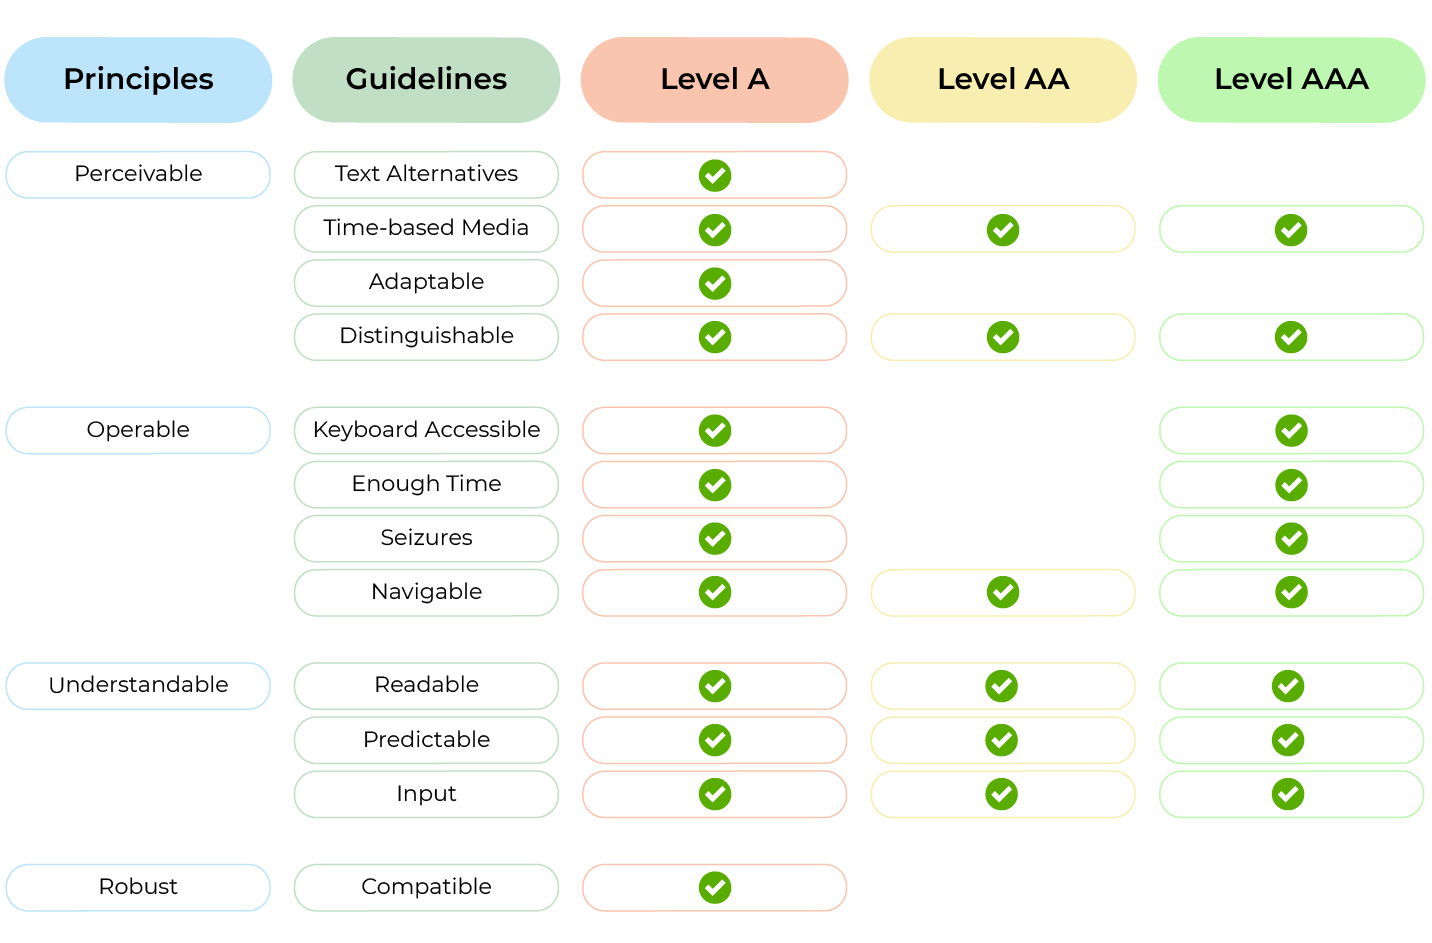
\includegraphics[scale=0.1]{res/wcag.png}
\caption{Linee guida WCAG e relativi livelli di accessibilità}
\label{fig:wcag}
\end{figure}

\subsection{Accessibilità di una risorsa}
Una risorsa accessibile è creata e studiata per essere facilmente fruibile da un utente, indipendentemente dalla sua disabilità o dal formato della risorsa. Rendere accessibile una risorsa è più semplice nelle fasi iniziali della creazione. Quando parliamo di risorse online di diversi tipi (testuali, immagini, video, audio) ci sono alcune considerazioni che dobbiamo verificare in modo da offrire una risorsa accessibile per utenti diversi. Nel caso delle risorse testuali, il livello d'accessibilità di un documento dipende da:
\begin{itemize}
    \item \textit{struttura}: una struttura standardizzata di documenti migliora l'accessibilità, perché consente agli utenti di trovare i contenuti in una parte specifica della pagina, senza aver bisogno di leggere tutto il documento;
    \item \textit{intestazioni}: devono essere descrittivi e in un ordine coerente;
    \item \textit{floating elements}: vanno inseriti all'interno della sezione di appartenenza;
    \item \textit{risoluzione}: i documenti dovrebbero essere accessibili ai lettori che utilizzano dispositivi con schermi piccoli o ai lettori che utilizzano monitor a bassa risoluzione;
    \item \textit{testo}: le dimensioni dei caratteri ridotti o ingranditi, il tipo dei caratteri, l'indentazione e lo spazio sono parametri che dovrebbero essere utilizzati in modo da creare un stile da rispettare per il documento e ciò migliora l'accessibilità della risorsa;
    \item \textit{colori}: definiscono un alto livello di accessibilità se definiti con accuratezza, ma non utilizzare testo o sfondo colorato perché lettori non vedenti che accedono tale risorsa tramite una stampa o un dispositivo senza schermo a colori non riceveranno tali informazioni;
    \item \textit{blocchi di elementi}: gli elementi dell'elenco non si devono separare lasciando righe vuote o interruzioni di colonna tabulari tra di loro;
\end{itemize}

Le immagini che non sono puramente decorative dovrebbero includere un attributo \textit{alt} che sostituisce l'informazione dell'immagine per i lettori non vedenti. Per le immagini è una buona prassi includere una didascalia utilizzando la sintassi dell'immagine incorporata, descrivendo in modo conciso il significato dell'immagine e le informazioni essenziali che trasmette. Il posizionamento delle immagini può essere diverso in base al dispositivo o al formato del documento e per questo motivo si deve evitare il riferimento statico delle immagini basato sulla posizione e utilizzare invece le didascalie per identificarle.

Nel caso di una risorsa multimediale, audio o video, è possibile aumentare l'accessibilità attraverso l'aggiunta dei sottotitoli in un formato di testo temporizzato, scaricabile a parte, contenente la trascrizione delle informazioni sonore.

\subsubsection{Leggibilità dei caratteri}
Durante la lettura del testo, la maggior parte delle persone non legge o analizza le singole parole, ma scansiona rapidamente il testo e analizza schemi e gruppi di caratteri (in genere 6-9 caratteri alla volta) a cui il cervello umano assegna un significato. Questo processo inconscio ci consente di leggere e comprendere il contenuto del testo molto rapidamente con alti gradi di comprensione, anche se non stiamo nemmeno vedendo o pensando a caratteri e parole.

È solo quando i caratteri o le parole non sono familiari o introducono una barriera a questo processo è necessario fermarsi per esaminare o elaborare più da vicino i caratteri o le parole. Per una leggibilità e una comprensibilità ottimali, è fondamentale evitare tali interruzioni.

\subsection{LOM}
Lo standard \textbf{IEEE LOM} o \textbf{LOM} (Learning Object Metadata) è uno standard aperto che
specifica la sintassi e la semantica degli attributi richiesti per i metadati dei learning object. Lo standard LOM include regole per controllare l'identificazione degli elementi dei dati e dei loro attributi. Fornisce inoltre principi, regole e strutture per la specificazione di quelle stesse risorse. Il suo obiettivo è facilitare la ricerca, la valutazione, il recupero e l'uso dei learning object.

Inoltre, IEEE LOM è considerato lo standard più accettato e implementato in più repository di learning objects. Esistono numerose versioni ed estensioni di LOM che sono state sviluppate da IEEE LOM. È organizzato in 9 categorie, ognuna delle quali contiene sottocategorie che possono condividere caratteristiche di base:

\begin{itemize}
\item \textit{Generale (general)} - 11 campi: racchiude le informazioni generali sui learning object;
\item \textit{Ciclo di vita (lifecycle)} - 6 campi: racchiude le informazioni sulla vita del learning object (versione, data di creazione, ecc.);
\item \textit{Meta-metadati (meta-metadata)} - 9 campi: fornisce informazioni sullo schema di metadati adottato;
\item \textit{Tecnico (technical)} - 12 campi: contiene informazioni sui requisiti e le caratteristiche tecniche del learning object;
\item \textit{Didattico (educational)} - 11 campi: racchiude informazioni sulle proprietà didattiche del learning object;
\item \textit{Diritti (rights)} - 3 campi: fornisce informazioni sui diritti intellettuali e simili del learning object;
\item \textit{Relazioni (relation)} - 7 campi: contiene indicazioni sul legame tra l'oggetto e altri oggetti o risorse;
\item \textit{Annotazioni (annotation)} - 3 campi: contiene commenti sull'uso didattico del learning object;
\item \textit{Classificazioni (classification)} - 8 campi: fornisce informazioni sul soggetto o la materia curricolare affrontata nel learning object.
\end{itemize}

\begin{figure}[H]
\centering
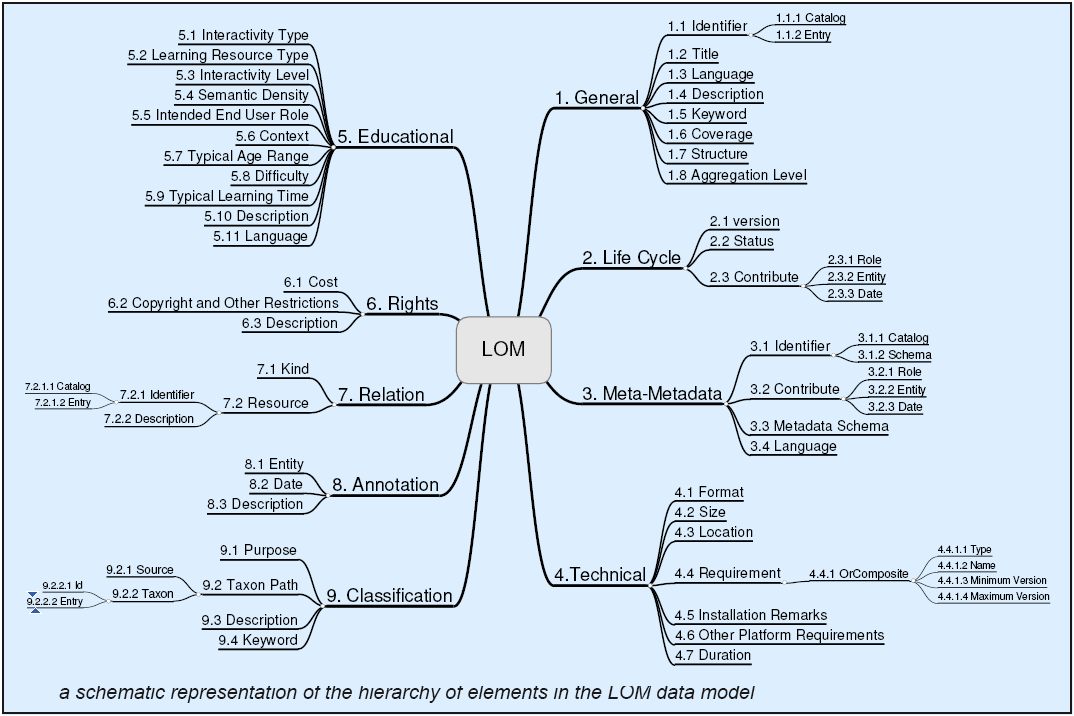
\includegraphics[scale=0.3]{res/LOM.png}
\caption{Gerarchia degli elementi del modello LOM}
\label{fig:lom}
\end{figure}

\subsection{LRMI}
Questa iniziativa è iniziata nel 2011, il suo scopo era quello di sviluppare una specifica come estensione didattica per Schema.org. Le proprietà LRMI hanno lo scopo di descrivere le risorse didattiche aggiungendo proprietà specifiche in modo che possano essere facilmente individuate attraverso motori di ricerca e servizi. Le specifiche si basano sul vocabolario fornito da Schema.org e da altri standard. Pertanto, ci sono termini LRMI non inclusi in Schema.org. 

Con il supporto di Association of Educational Publishers (AEP), Association of American Publishers, Creative Commons (CC), division 501, Bill \& Melinda Gates e William and Flora Hewlett Foundation, LRMI ha sviluppato un framework di metadati per taggare le risorse di apprendimento web. Lo schema LRMI 1.1 è stato adottato da Schema.org nel 2013, che consente alle risorse, attraverso i loro metadati LRMI, di essere riconosciute dai principali motori di ricerca.

Utilizza prevalentemente proprietà di risorse di tipo \texttt{Schema.org/CreativeWork} che sono state proposte a Schema.org da LRMI per descrivere le caratteristiche educative delle risorse di apprendimento. Per alcune di queste proprietà utilizza i tipi creati da LRMI \texttt{Schema.org/AligmentObject} e \texttt{Schema.org/EducationalAudience}.

Proprietà aggiunte da LRMI a \texttt{Schema.org/CreativeWork}, che rappresenta un generico lavoro creativo (libro, film, foto, programma software, ecc.):
\begin{itemize}
\item \texttt{educationalAligment}: quadro educativo stabilito
\item \texttt{educationalUse}: scopo del lavoro nel contesto dell'istruzione
\item \texttt{timeRequired}: tempo approssimativo necessario per lavorare sulla risorsa
\item \texttt{typicalAgeRange}: fascia di età dell'utente finale
\item \texttt{interactivityType}: attivo, espositivo o misto
\item \texttt{learningResourceType}: tipo di risorsa predominante (presentazione, brochure, ecc.)
\item \texttt{useRightsUrl}: URL in cui vengono stabilite le autorizzazioni per l'utilizzo delle risorse
\item \texttt{isBasedOnUrl}: risorsa utilizzata per la creazione
\end{itemize}

Proprietà aggiunte da LRMI a \texttt{Schema.org/Intangibles/AligmentObject}, un elemento immateriale che descrive un allineamento tra una risorsa di apprendimento e un nodo in un framework didattico:
\begin{itemize}
\item \texttt{aligmentType}: allineamento tra la risorsa di apprendimento e il nodo del framework. I valori consigliati includono: 'evaluate', 'teach', 'require', 'textComplexity', 'readingLevel', 'educationalSubject', and 'educationLevel'
\item \texttt{educationalFramework}: framework per la descrizione delle risorse
\item \texttt{targetDescription}: descrizione del nodo di un framework didattico
\item \texttt{targetName}: nome del nodo di un framework didattico
\item \texttt{targetUrl}: URL di un nodo di un framework didattico
\end{itemize}

Proprietà aggiunte da LRMI a \texttt{Schema.org/Audence/EducationalAudience}:
\begin{itemize}
\item \texttt{EducationalRole}: pubblico di destinazione
\end{itemize}

\subsection{IMS AfA}
L'obiettivo principale di IMS Access for All (\textbf{AfA}) v3.0 era quello di semplificare lo standard ISO/IEC 24751 a causa delle difficoltà sorte nella pratica. Entrambi, lo standard ISO/IEC 24751 e AfA v3.0, coprono l'intero processo dalla lettura delle esigenze dell'utente al meccanismo di ricerca necessario per trovare i learning object che soddisfano tali esigenze o preferenze. Ha due modelli di dati:
\begin{itemize}
\item Personal Needs and Preferences (PNP): un modello per la descrizione dei bisogni e delle preferenze degli utenti per accedere e interagire con le risorse digitali.
\item Digital Resource Description (DRD): un modello per la descrizione dei metadati di accessibilità per le risorse didattiche digitali.
\end{itemize}

La specifica AfA DRD definisce i metadati di accessibilità per una risorsa che verrà utilizzata per la ricerca e l'uso della risorsa di apprendimento più adatta per ciascun utente secondo i PNP. Lo strumento LOMPAD è stato abilitato per introdurre metadati di accessibilità (oltre ai metadati ordinari) secondo la specifica IMS 3.0.

Il modo di lavorare con oggetti di apprendimento accessibili richiede la creazione di oggetti di apprendimento originali e adattati. Esistono diversi strumenti che ne facilitano la creazione. Una risorsa originale corrisponde a una risorsa iniziale, mentre una risorsa adattata presenta le stesse informazioni didattiche della risorsa iniziale o originale ma con caratteristiche diverse, come la modalità sensoriale di accesso alla risorsa, la lingua, ecc. Ad esempio, un file in formato pdf come risorsa originale e una descrizione audio del suo contenuto come risorsa adattata. Il primo presenta l'accesso testuale mentre l'adattamento presenta l'accesso uditivo allo stesso contenuto didattico. Pertanto, le risorse originali possono avere un numero qualsiasi di adattamenti, totali o parziali.

I metadati possono supportare le informazioni adeguate delle risorse originali, come la modalità di accesso (vista, udito, alfabetizzazione, presentazione, fattibilità della trasformazione, controllo, flessibilità, adattamenti, strumenti di aiuto, ecc.) e informazioni rilevanti sulle risorse adattate, come il tipo di adattamento (sottotitoli, lingua dei segni), l'estensione, e la descrizione. Una fusione di risorse, metadati descrittivi e metadati di accessibilità corrisponde al consolidamento di una fonte di archivi accessibili che rafforzi la ricerca di learning object secondo i bisogni educativi speciali.

\begin{figure}[H]
\centering
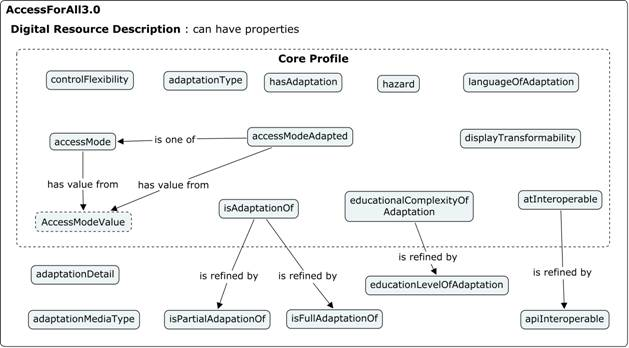
\includegraphics[scale=0.7]{res/drd.png}
\caption{Proprietà del modello DRD}
\label{fig:drd}
\end{figure}

Lo scopo della specifica AfA PNP è quello di consentire la definizione dei bisogni personali degli studenti (o quelli relativi agli ambienti della disabilità). I PNP vengono utilizzati in combinazione con la specifica AfA DRD per fornire risorse digitali che soddisfino le esigenze di un utente e/o le sue preferenze. I PNP dello studente o dell'utente definiscono le sue preferenze nell'utilizzo delle diverse modalità sensoriali per la percezione delle informazioni. Il metodo suggerito per generare i PNP dello studente è la presentazione di un modulo con diverse opzioni sulla modalità sensoriale preferita per l'accesso alle informazioni. I PNP saranno generati dalle risposte dello studente alle domande nel modulo.

I principi di accessibilità sull'e-learning sono focalizzati sulla fornitura di opzioni di personalizzazione basate sulle preferenze dell'utente, sugli equivalenti dei contenuti e sulla compatibilità con l'aiuto tecnico e l'accesso completo alla tastiera, oltre a fornire informazioni sul contesto e offrire supporto in modo che l'utente possa seguire specifiche su direttive e/o norme di organi di governo come IMS.

\begin{figure}[H]
\centering
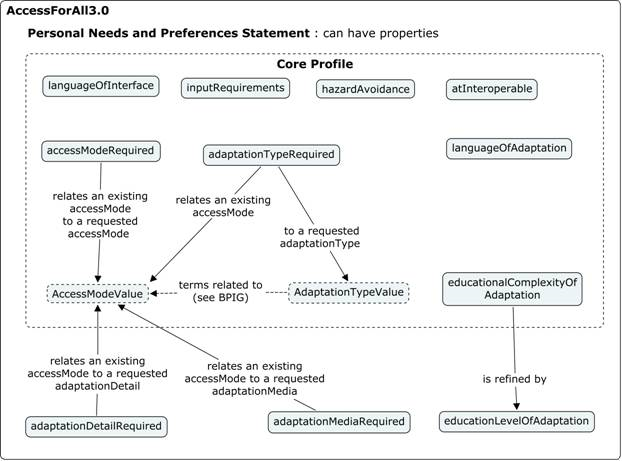
\includegraphics[scale=0.7]{res/pnp.png}
\caption{Proprietà del modello PNP}
\label{fig:pnp}
\end{figure}

\subsection{Schema.org}
\textbf{Schema.org} è una comunità responsabile della creazione, della manutenzione e della promozione di schemi di metadati per dati strutturati pubblicati su Internet. L'aspetto più interessante di Schema.org è che riceve il supporto di grandi aziende come Google, Microsoft e Yahoo. Ciò significa che l'incorporazione di metadati nei contenuti pubblicati su Internet è essenziale per poterli categorizzare e descrivere le loro caratteristiche di accessibilità.

I formati più utilizzati per fare annotazioni semantiche sono microdati, microformati, JSON-LD e RDFa.
Il formato dei microdati è stato sviluppato nell'ambito della standardizzazione di HTML5 per la marcatura dei contenuti web. I microdati sono costituiti da un gruppo di coppie nome-valore; i gruppi sono chiamati elementi e ogni coppia nome-valore è una proprietà. Gli elementi sono definiti dai seguenti cinque attributi: \textit{itemscope}, \textit{itemtype}, \textit{itemid}, \textit{itemprop} e \textit{itemref}. Queste annotazioni forniscono la semantica attraverso la terminologia e le proprietà di un dominio di rappresentazione della conoscenza, comprese le sue relazioni.

La specifica Schema.org stabilisce una raccolta di vocabolari condivisi che includono proprietà per descrivere alcune caratteristiche di diversi tipi di contenuto web. Queste descrizioni possono essere comprese dai principali motori di ricerca. Nel caso di Google, il suo motore di ricerca utilizza i microdati HTML5 di Schema.org per migliorare i risultati delle sue ricerche e consente a chiunque di effettuare una ricerca personalizzata utilizzando i diversi schemi di Schema.org per limitare le ricerche.

Per definire i metadati di accessibilità in Schema.org, sono definiti diversi tipi di contenuto web e possono essere
classificati utilizzando schemi di metadati.
I tipi possono avere sottotipi, ad esempio "CreativeWork" ha il tipo "MediaObject" e questo ha a sua volta "VideoObject".
I metadati di accessibilità definiti da Schema.org si basano su quelli specificati per IMS AfA v3.0 DRD, ma ne è stato selezionato un sottoinsieme significativo. Ciascuno di questi metadati può avere un possibile valore definito nella specifica. In questo modo si possono determinare le caratteristiche di accessibilità di qualsiasi risorsa digitale pubblicata sul web.

\begin{figure}[H]
\centering
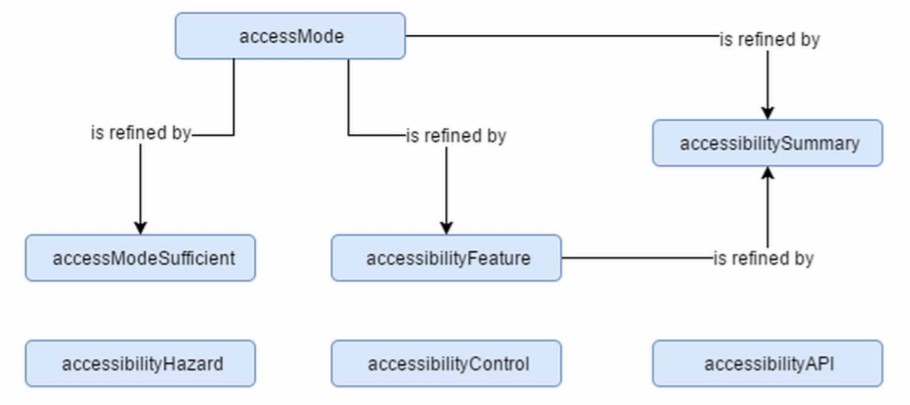
\includegraphics[scale=0.7]{res/schemaorg.png}
\caption{Metadati di accessibilità di CreativeWork da Schema.org}
\label{fig:schemaorg}
\end{figure}

\subsection{AccessibleOCW}
AccessibleOCW è un ontologia sviluppata da OCW (\textit{OpenCourseWare}) per rappresentare l'accessibilità e gli adattamenti delle risorse digitali nell'ambito dell'e-learning.

L'ontologia ha specificato un insieme di classi per la modellazione dell'accessibilità e l'adattamento del formato delle risorse, tra le quali:
\begin{itemize}
    \item \texttt{AdaptationDetailRequired}: il tipo di adattamento obbligatorio dei dettagli di una risorsa;
    \item \texttt{AdaptationDetailValue}: diversi tipi di adattamento dei dettagli di una risorsa;
    \item \texttt{AdaptationMediaRequired}: il tipi adattamento obbligatorio del formato audio-visivo della risorsa;
    \item \texttt{AdaptationMediaTypeValue}: diversi tipi di adattamento del formato audio-visivo della risorsa;
    \item \texttt{AdaptationTypeValue}: diversi tipi di adattamento di una risorsa (ad esempio testo alternativo per le immagini, descrizione testuale per le risorse audio, didascalie per le risorse video, etc);
    \item \texttt{ControlFlexibilityValue}: rappresenta la flessibilità con il controllo dei dispositivi elettronici (ad esempio tastiera, mouse, etc);
    \item \texttt{DisplayTransformabilityValue}: rappresenta le trasformazioni che si possono effettuare ad una risorsa in modo da aumentare il suo livello d' accessibilità (ad esempio colore del background, font size, font weight, etc);
    \item \texttt{EducationalComplexityValue}: modella il livello di complessità di una risorsa;
\end{itemize}

	\clearpage{\pagestyle{empty}\cleardoublepage}
\chapter{Contesto del progetto}
\textbf{Pathadora} è un sistema di raccomandazione progettato per suggerire agli studenti le facoltà e i corsi più idonei per loro sulla base delle informazioni specificate, sia personali che relative a eventuali disabilità possedute. 

Pathadora può essere suddiviso in due sottosistemi: 
\begin{itemize}
\item \textbf{Pathadora Recommender}, che memorizza le entità del dominio in un'ontologia del web semantico (\textit{Pathadora Ontology}) e produrrà i risultati relative a facoltà, corsi e risorse suggeriti utilizzando regole SWRL e SPARQL (\textit{Pathadora Rule Model}). Le operazioni vengono eseguite a seguito delle richieste HTTP ricevute dalla web app, intercettate mediante un server back-end (\textit{Pathadora Engine}).

Per permettere le interrogazioni su una grande quantità di dati è stato progettato un knowledge graph mediante la piattaforma \textbf{Stardog}. Un knowledge graph consiste nell'applicazione del modello descritto dall'ontologia su un insieme di istanze, \textit{individual}, collegati tra loro mediante relazioni.
\item \textbf{Pathadora Web App}, permette all'utente di interfacciarsi con Pathadora Recommender creando un proprio profilo per poi sottomere richieste per ottenere risultati su facoltà, corsi e risorse didattiche suggerite. Permette inoltre la registrazione di profili per docenti, i quali possono caricare le risorse didattiche relative ai propri corsi per cui, quando possibile, verranno generati metadati relativi all'accessibilità del contenuto; queste verranno poi utilizzati dal sistema di raccomandazione per determinare se suggerire o meno la risorsa associata a utenti con determinate disabilità.
\end{itemize}

\begin{figure}[H]
\centering
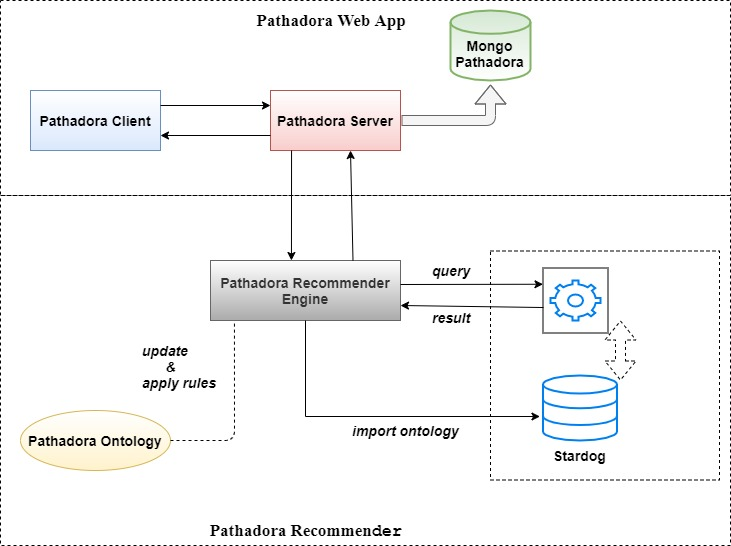
\includegraphics[scale=0.4]{res/pathadora-arch.jpg}
\caption{Architettura di Pathadora}
\label{fig:pathadora-arch}
\end{figure}

\begin{figure}[H]
\centering
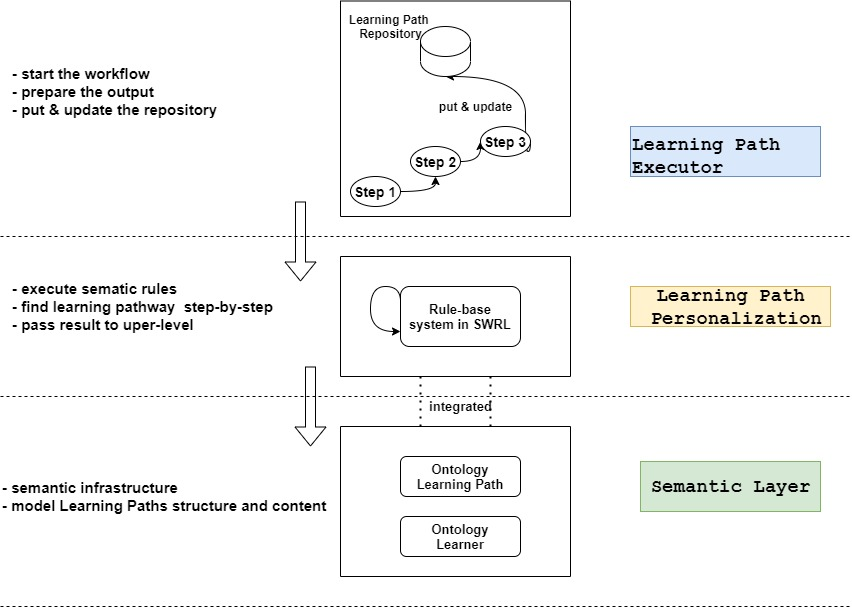
\includegraphics[scale=0.4]{res/diag-layers.jpg}
\caption{Workflow del sistema di raccomandazione}
\label{fig:diag-layers}
\end{figure}

\begin{figure}[H]
\centering
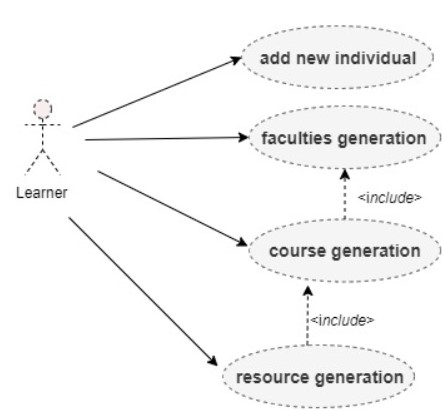
\includegraphics[scale=0.4]{res/pathadora-engine.jpg}
\caption{Casi d'uso sul Pathadora Recommender Engine}
\label{fig:pathadora-engine}
\end{figure}

\subsection{Richieste}
L'interfaccia web permette l'invio di richieste da sottomettere al Pathadora Engine attraverso appositi form.

\subsubsection{Inserimento}
La prima tipologia di richiesta da gestire è l'inserimento di nuove istanze nell'ontologia. In questa richiesta dovranno essere specificate tutte le informazioni che serviranno all'engine per aggiornare il knowledge graph. La richiesta potrebbe dichiarare relazioni tra elementi che non sono presenti e in tal caso, l'engine prima creerà questi elementi per poi definire la relazione tra
loro. Nel caso della richiesta di inserimento tutti gli elementi verranno aggiunti nell'ontologia, indipendentemente se esistono, se rispettano il formato giusto oppure se le relazioni sono semanticamente corrette.

\paragraph{Inserimento learner}
Alla registrazione di uno studente corrisponderà l'inserimento di un individual Learner nell'ontologia, le cui proprietà verranno utilizzate dal sistema per suggerire facoltà, corsi e risorse allo studente.

Le informazioni inserite riguardano le lingue conosciute, i titoli di laurea corrente e futuro, le passioni per determinati settori, gli obiettivi dello studente e il possedimento di determinate disabilità con relativi livelli associati.

\begin{figure}[H]
\centering
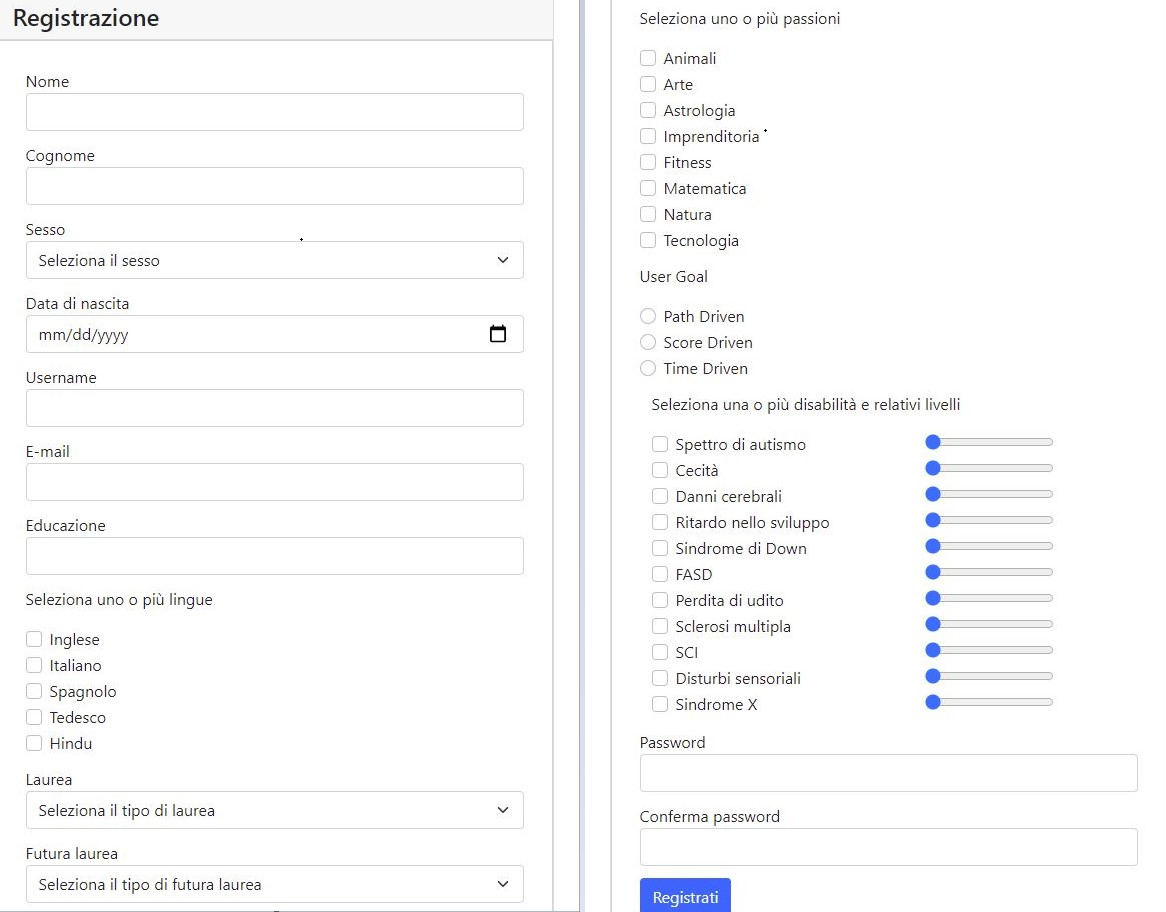
\includegraphics[scale=0.4]{res/registrazione.jpg}
\caption{Form di registrazione studente}
\label{fig:registration}
\end{figure}

\paragraph{Inserimento corsi}
Un docente registrato può personalizzare il suo profilo modificando le informazioni associate ai corsi di cui è titolare. I corsi inseriti saranno visualizzablii dagli studenti in una finestra dedicata.

Le informazioni associate al corso riguardano la lingua, il semestre di appartenenza, i CFU, l'anno, la tipologia (triennale, magistrale, dottorato), l'area scientifica di appartenenza e l'obbligatorietà del corso.

\paragraph{Inserimento risorse}
I docenti possono aggiungere risorse didattiche ai corsi a cui sono associati, descrivendoli con informazioni relative alla loro accessibilità.

Le informazioni sono relative al tipo di adattamento, al grado di trasformazione applicabile su determinati elementi del contenuto (dimensione del testo), alla modalità di accesso e al tipo di risorsa. Verranno inoltre generati automaticamente indicatori numerici relativi al grado di leggibilità del testo contenuto in una risorsa, del rapporto di contrasto tra il colore del testo contenuto nelle immagini di un documento e relativo colore di sfondo, e della dimensione dei caratteri minima presente nel documento.

Le risorse potranno essere consultabili dagli studenti nella schermata dedicata ai corsi.

\subsubsection{Generazione di dipartimenti e facoltà}
A seguito della registrazione, lo studente può richiedere la generazione dei dipartimenti e delle facoltà suggerite. I risultati dipenderanno dalla corrispondenza tra le passioni dello studente e l'area scientifica di appartenenza dei dipartimenti e quindi delle facoltà, oltre che dal tipo di laurea (triennale, magistrale, dottorato) a cui lo studente ambisce.

\begin{figure}[H]
\centering
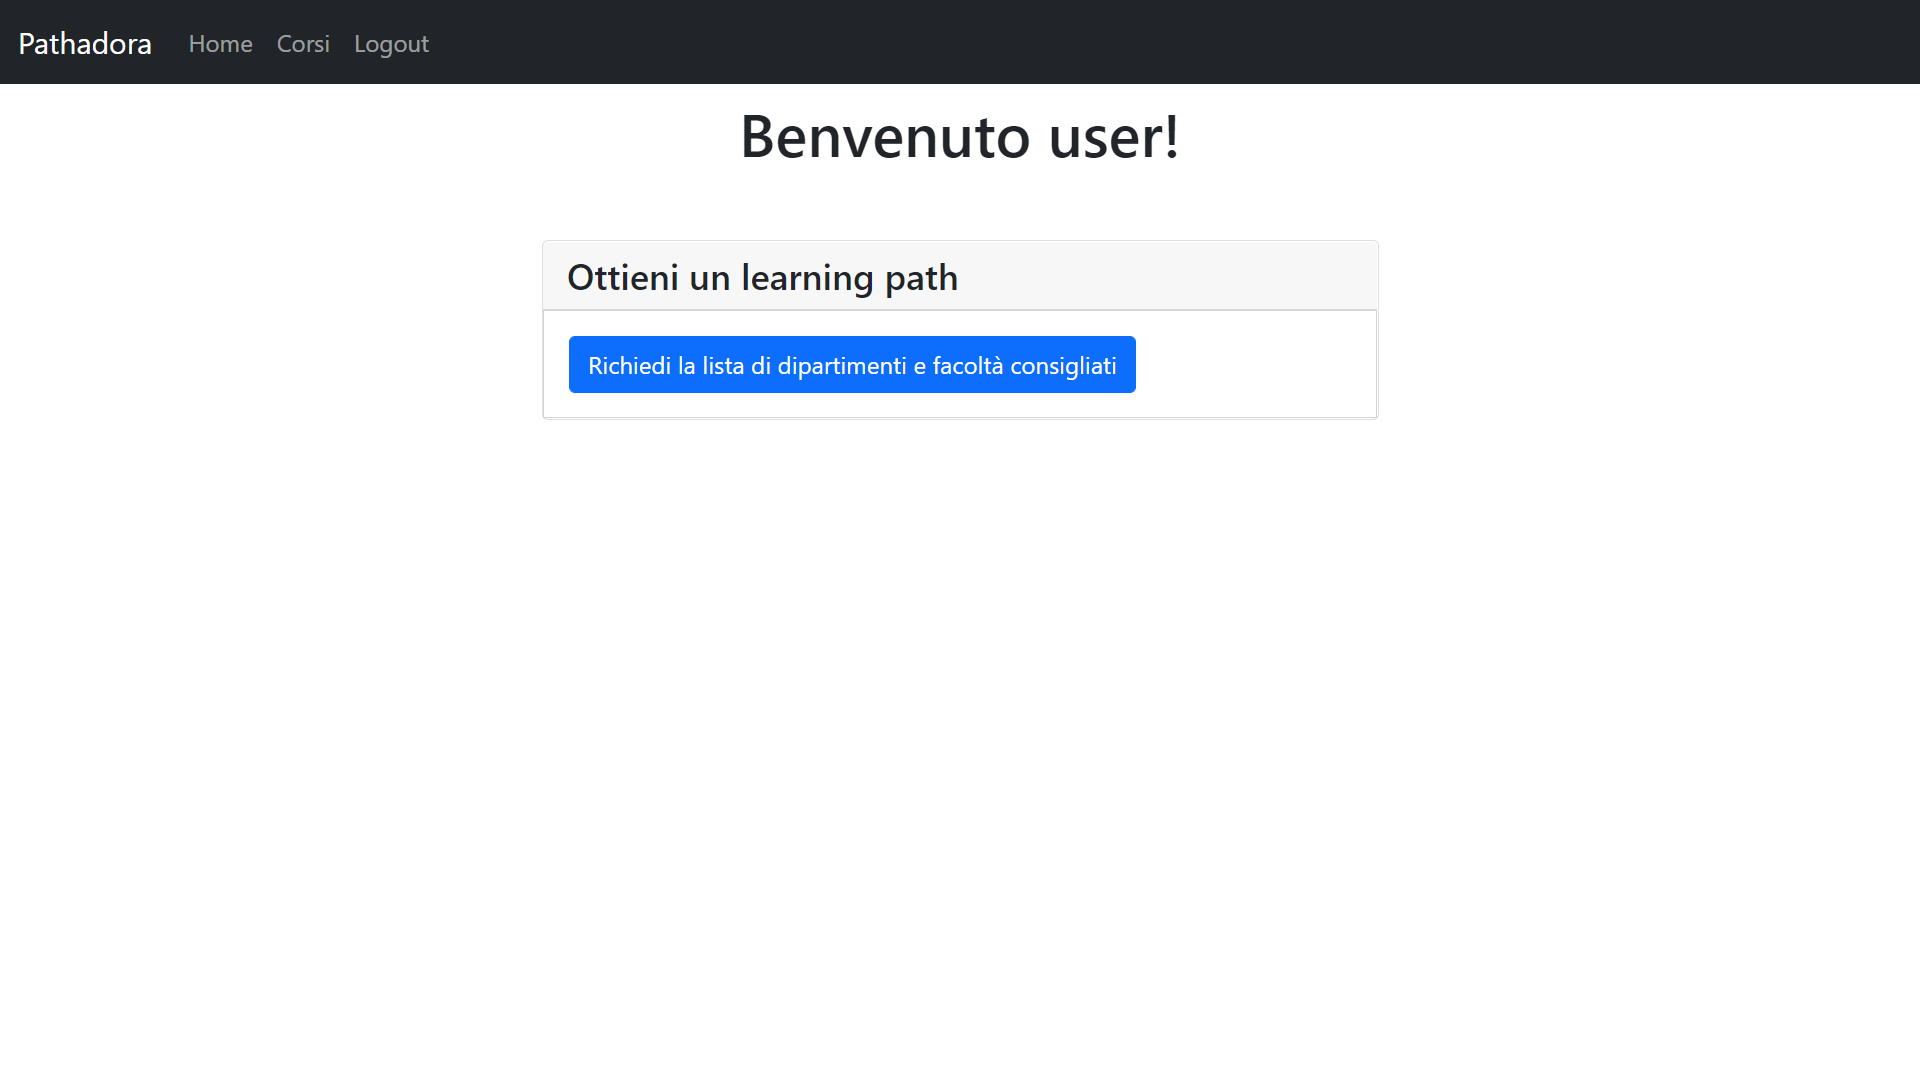
\includegraphics[scale=0.4]{res/faculties-generation.png}
\caption{Form di richiesta dipartimenti e facoltà suggeriti}
\label{fig:faculties-generation}
\end{figure}

\subsubsection{Generazione di corsi}
Una volta generate le facoltà, lo studente può richiedere la generazione dei corsi suggeriti selezionando la facoltà e l'anno preferiti. 
Una volta ricevuto tale scelta, il sistema inizializzerà il knowledge graph e lo interrogherà parametrizzando la query con le informazioni dello studente.

\begin{figure}[H]
\centering
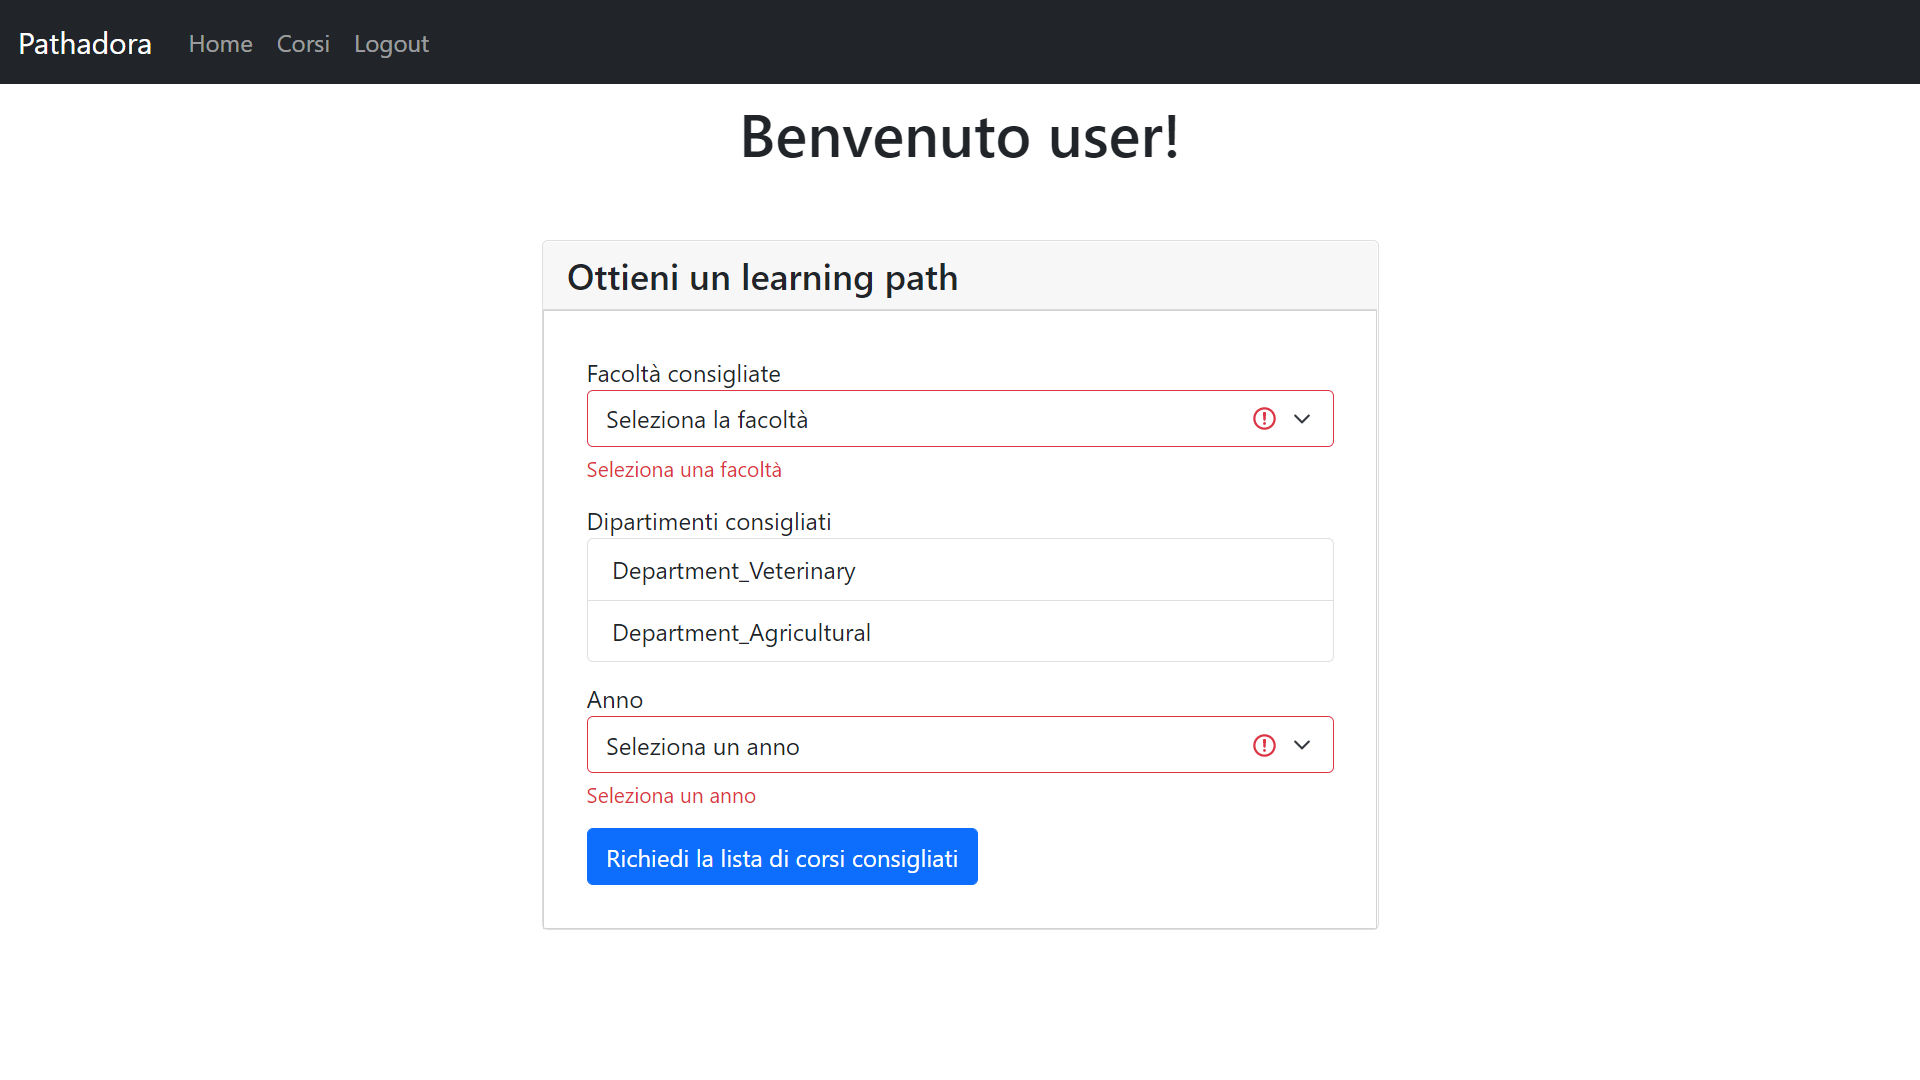
\includegraphics[scale=0.4]{res/courses-generation.png}
\caption{Form di richiesta corsi suggeriti}
\label{fig:courses-generation}
\end{figure}

\subsubsection{Generazione di risorse}
L'ultima richiesta da gestire consiste nella raccomandazione delle risorse relative a un corso specifico tra quelli suggeriti, risultati della richiesta precedente.
La raccomandazione terrà conto delle disabilità dello studente per determinare le risorse da raccomandare allo studente, a cui possono essere associate informazioni relative all'accessibilità come il grado di leggibilità del testo e la dimensione minima del font di un documento.

\begin{figure}[H]
\centering
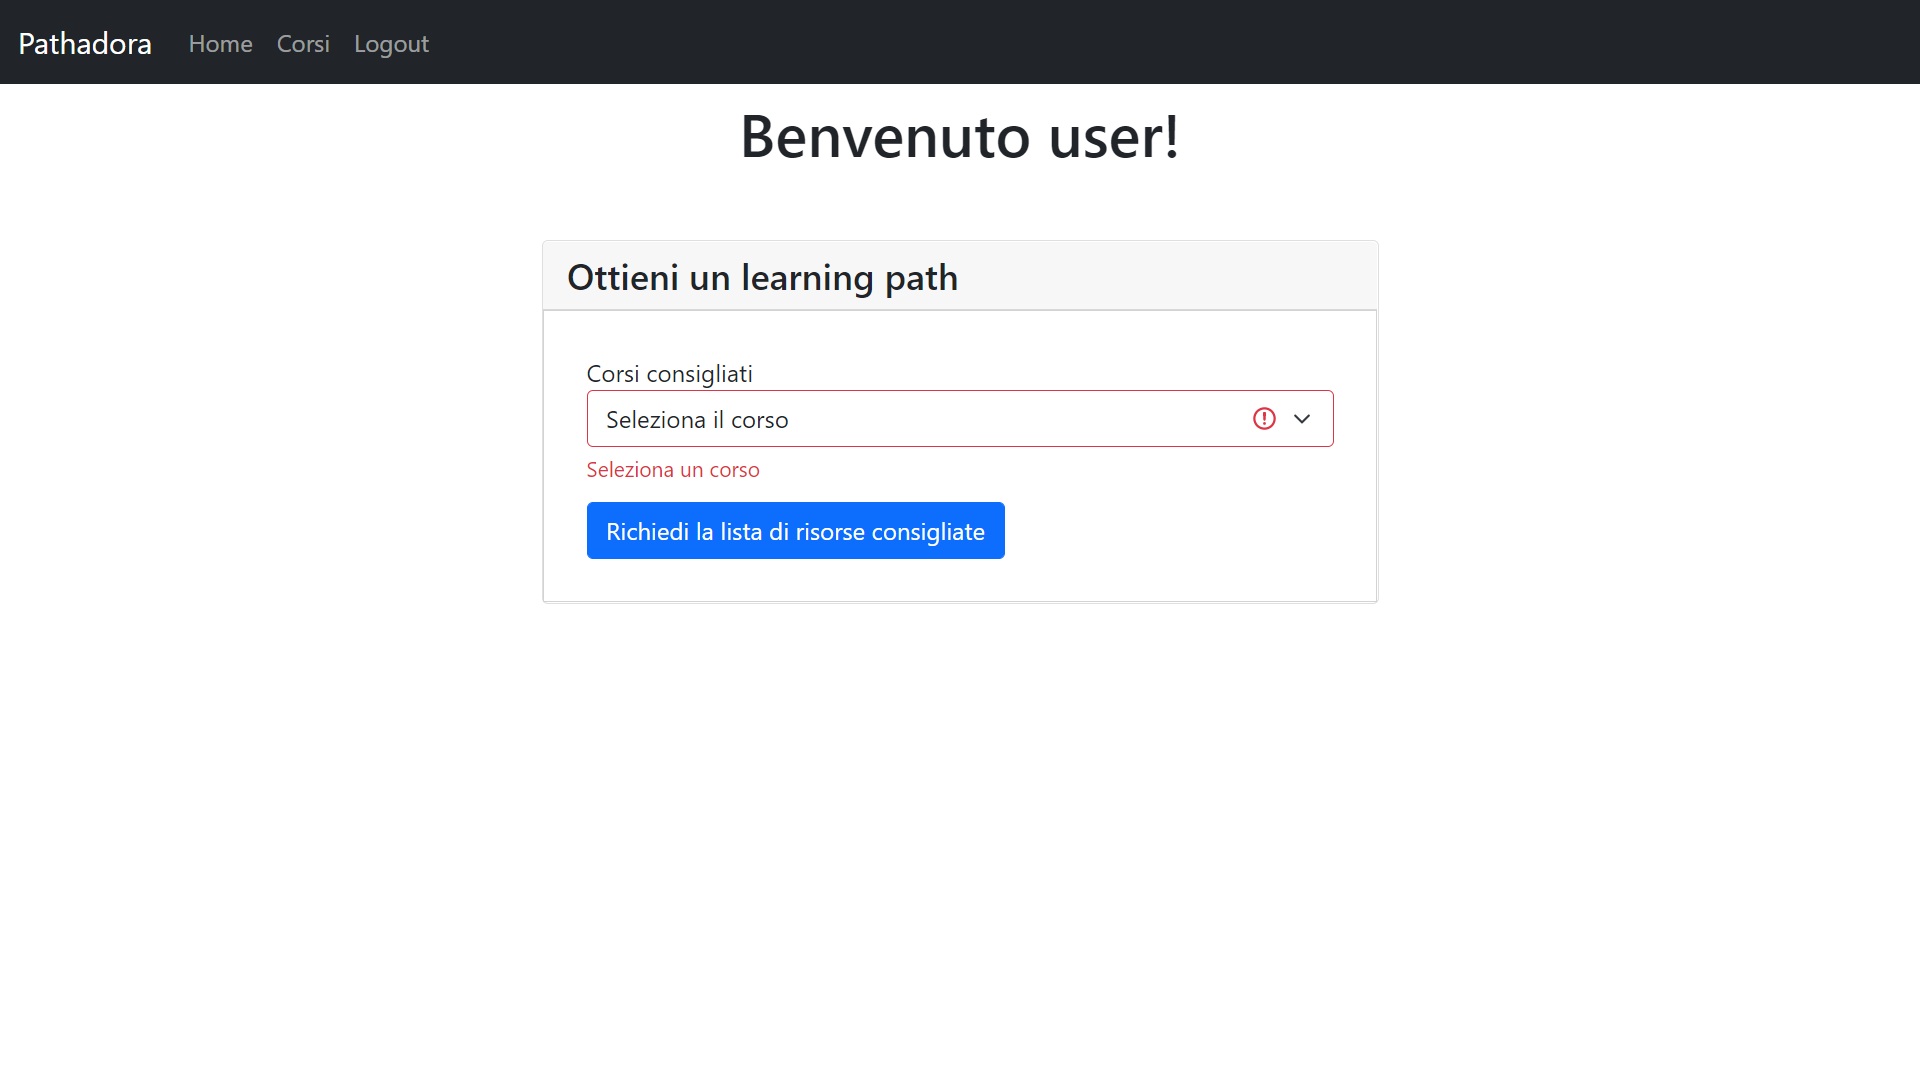
\includegraphics[scale=0.4]{res/resources-generation.png}
\caption{Form di richiesta risorse suggerite}
\label{fig:resources-generation}
\end{figure}

\begin{figure}[H]
\centering
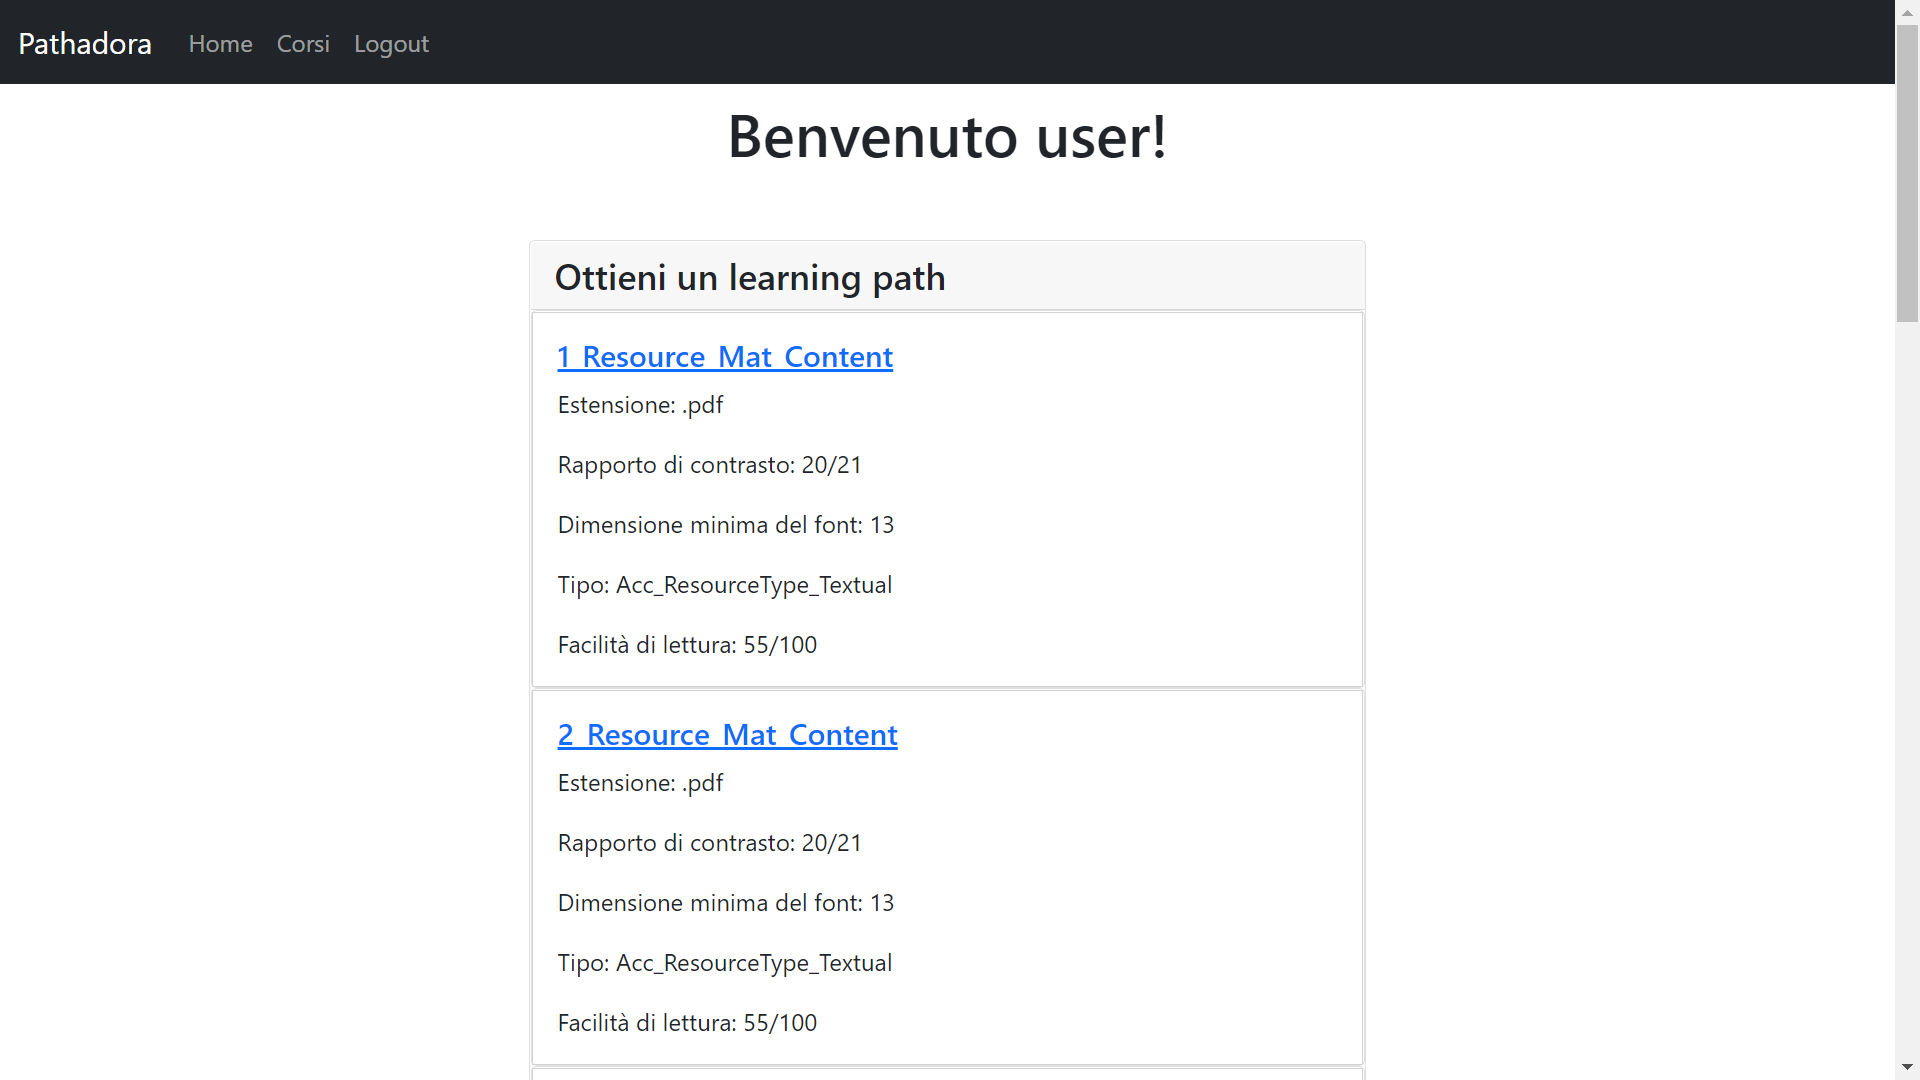
\includegraphics[scale=0.4]{res/path-result.png}
\caption{Risultato risorse suggerite}
\label{fig:resources-generation}
\end{figure}

\subsection{Ontologia}
L'ontologia \texttt{pathadora-ontology} racchiude tutti i concetti del sistema, importando altre ontologie pubbliche come \texttt{LOM} e \texttt{AccessibleOCW}, in modo da offrire un modello completo per la rappresentazione della conoscenza.

\subsubsection{Learner}
L'entità \texttt{Learner} modellata in Pathadora è lo stesso concetto rappresentato nell'ontologia \texttt{AccessibleOCW}. A tale entità vengono aggiunte altre proprietà per definire semanticamente le sue caratteristiche.

Tramite la proprietà \texttt{hasDegree}, l'ontologia permette di modellare i diplomi conferiti dallo studente. La proprietà \texttt{futureDegree} mette in relazione lo studente con il tipo di diploma che vorrebbe conseguire in futuro. Tramite \texttt{hasGoals}, l'ontologia modella gli obiettivi dello studente e fornisce anche delle sottoproprietà basandosi sul tipo dell'obiettivo (ad esempio \texttt{isPathDriven}, \texttt{isScoreDriven}, \texttt{isTimeDriven}, ecc.). Lo stile d'apprendimento di uno studente viene specificato tramite la proprietà \texttt{learningStyle}. Come nel caso degli obiettivi, anche le passioni vengono modellate tramite la proprietà \texttt{passionateOf} e le sottoproprietà in base alla tipo della passione. Le informazioni che riguardano le lingue che uno studente potrebbe parare vengono inserite tramite la proprietà \texttt{speaks}.
La proprietà \texttt{hasDisability} rappresenta le informazioni che riguardano le disabilità dello studente e come range di valori aspetta un'istanza della classe \texttt{Disabilities}.

\subsubsection{University}
L'organizzazione di tale istituzione viene rappresentata tramite una gerarchia di classi. I dipartimenti associati ad una scuola vengono messi in relazione tramite la proprietà \texttt{departmentOf}, mentre le facoltà di un dipartimento vengono specificate tramite \texttt{facultyOfDepartment}. Seguendo la stessa logica, i corsi vengono associati ad una facoltà tramite la proprietà \texttt{courseOfFaculty}. La proprietà \texttt{courseLanguage} permette di specificare in quale lingue verranno tenute le lezione di un corso. Un determinato corso viene dichiarato come obbligatorio oppure opzionale tramite la proprietà \texttt{isCourseObligatory} avendo come range un tipo di dato \texttt{boolean}. Le proprietà \texttt{courseSSD} e \texttt{courseType} mettono in relazione rispettivamente un corso con il suo tipo e il suo settore scientifico. Il range di queste due proprietà deve essere un istanza delle classi \texttt{CourseSSD} e \texttt{CourseType}. 

Per le istanze che rappresentano i corsi, sono state definite un insieme di proprietà dei dati tra le quali:
\begin{itemize}
    \item \texttt{coursePeriod}: specifica il periodo del corso;
    \item \texttt{courseCFU}: specifica i CFU del corso;
    \item \texttt{courseYear}: specifica l'anno del corso;
\end{itemize}

\subsubsection{LearningObject}
Pathadora unisce le modellazioni del concetto di risorsa didattica delle ontologie \texttt{LOM} e \texttt{AccessibleOCW}, rispettivamente focalizzati sulle informazioni di natura generale e sui diversi tipi di accessibilità che la risorsa possiede.

Vengono inoltre aggiunte ulteriori proprietà che descrivono il livello dell'accessibilità, mappando la modalità d'accesso ad un risorsa con un tipo di dato numerico:
\begin{itemize}
    \item \texttt{resourceContrastRatio}: coefficiente che rappresenta il contrasto visivo della risorsa con range 1-100;
    \item \texttt{resourceReadingEase}: coefficiente con range 1-100 che specifica il grado di leggibilità di una risorsa;
    \item \texttt{resourceFontSize}: specifica la dimensione del font minima del testo e lo mappa in un coefficiente d'accessibilità;
\end{itemize}

L'ontologia, tramite la proprietà \texttt{resourceType}, associa ad una risorsa il tipo (testuale, video, audio, immagine, ecc.).

\subsubsection{Disabilities}
Pathadora si basa sull'ontologia \texttt{AccessibleOCW} per modellare le disabilità di uno studente.
Vengono inoltre modellati attraverso valori numerici con range da 1 a 100 i livelli di disabilità dello studente (\texttt{autismSpectrumLevel}, \texttt{blindnessLevel}, \texttt{hearingLossLevel}, ecc.).
Durante la registrazione l'utente dovrebbe specificare questi livelli, anche stimarli in modo non preciso, per permettere al sistema di interpretali e mapparli con i coefficienti d'accessibilità delle risorse.

La proprietà \texttt{hasDisabilites} mette in relazione uno studente con un tipo di disabilità. Pathadora raggruppa le disabilità in diverse categorie che saranno istanze delle classi \texttt{Intellectual}, \texttt{Physical} e \texttt{Sensory}.
	\clearpage{\pagestyle{empty}\cleardoublepage}
\chapter{Tecnologie utilizzate}                %crea il capitolo
%%%%%%%%%%%%%%%%%%%%%%%%%%%%%%%%%%%%%%%%%imposta l'intestazione di pagina

\subsection{Angular}
\textbf{Angular} è un framework open source per lo sviluppo di applicazioni web scritto interamente in TypeScript.

Un elemento fondamentale per la costruzione di applicazioni Angular è il componente, al quale viene affidato il controllo di una porzione dello schermo, acquisendo la responsabilità di visualizzare i dati ricevuti e gestirne l’interazione con l’utente secondo il concetto di view.

Una moderna applicazione Angular è sintetizzabile in un insieme di componenti ordinate in modo gerarchico con le quali vengono fornite le funzionalità con cui far interagire l’utente.

Tra i principali motivi che rendono vantaggioso questo modello di programmazione vi è il fatto di poter assemblare applicazioni diverse utilizzando un insieme comune di componenti, favorendo quindi il riutilizzo del codice; al contempo la struttura definita dell’applicazione ne favorisce la suddivisione in moduli e la leggibilità del codice scritto.

\vspace{5mm}

Ogni componente ha un modello HTML che dichiara come quel componente viene visualizzato.

Angular estende l'HTML con una sintassi aggiuntiva che permette di inserire valori dinamici inizializzati nel componente. Angular aggiorna automaticamente il DOM renderizzato a ogni cambiamento dello stato del componente e seguendo le istruzioni fornite dalle cosiddette direttive. Questo modello di progettazione consente di scrivere codice più flessibile e testabile.

Angular inoltre fa uso del pattern dependency injection, che consente di dichiarare le dipendenze delle classi TypeScript lasciando gestire l'istanziazione interamente al framework. Quando Angular crea un componente, chiede all’injector i servizi richiesti. Un injector mantiene un container delle istanze dei servizi che sono stati precedentemente creati. Se un’istanza di un servizio richiesto non è nel container, l’injector ne crea uno e lo aggiunge al container.

\begin{figure}[H]
\centering
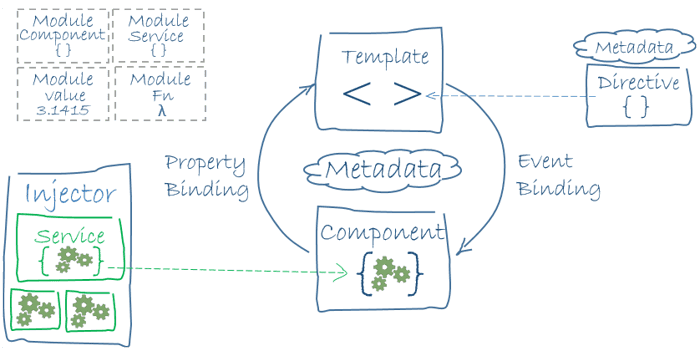
\includegraphics[scale=0.5]{res/angular.png}
\caption{Struttura di Angular}
\label{fig:angular}
\end{figure}

\subsubsection{Vantaggi e svantaggi}

Essendo basato su TypeScript, un linguaggio di programmazione che differisce da JavaScript e che offre numerose funzionalità aggiuntive come ad esempio la presenza di tipi statici, possono essere implementati numerosi tool per supportare meglio i programmatori e ridurre i bug nelle applicazioni.
Altra differenza importante è la presenza di numerose funzionalità aggiuntive come RxJS o la presenza stessa di un modello dei dati consistente integrato grazie al linguaggio Typescript, elemento assente ad esempio nel framework rivale React.

Al contempo l’onere di avere molte funzionalità integrate comporta un peso maggiore in termini di spazio di archiviazione in seguito alla prima installazione, mentre in altri concorrenti il peso effettivo del framework è decisamente inferiore, risultando
migliori per applicazioni meno complesse o che necessitano di meno funzionalità di quelle proposte da Angular.

Infine va rilevata una ridotta flessibilità del framework di Google rispetto ai rivali, con tutti i vantaggi e gli svantaggi derivanti da questa scelta soprattutto a livello progettuale. Un programmatore che sceglie Angular desidera una progettazione meno
impegnativa e approva tutte le scelte che il framework ha preso al posto suo; un programmatore di un altro framework desidera invece fare delle scelte personalizzate, dettate dalle proprie necessità progettuali, assumendosi poi però la responsabilità di mantenere aggiornate tutte le dipendenze inserite all’interno della propria applicazione.

\subsection{Bootstrap}
\textbf{Bootstrap} è un framework CSS gratuito e open source per la creazione di siti e applicazioni per il web. Contiene modelli di design basati su CSS e estensioni opzionali di JavaScript per tipografia, moduli, pulsanti, navigazione e altri componenti dell'interfaccia.

Tra le principali caratteristiche di questa libreria troviamo la piena compatibilità con tutte le ultime versioni di tutti i principali browser utilizzati, il supporto al responsive web design, l’adozione di una filosofia mobile-first per quanto riguarda il design oltre che un’ottima documentazione a corredo della libreria per rendere più facile la sua diffusione.

Gli sviluppatori possono sfruttare le classi CSS definite in Bootstrap per personalizzare ulteriormente l'aspetto dei loro contenuti.\cite{bootstrap}

\subsection{Node.js}
\textbf{Node.js} è un runtime JavaScript basato sugli eventi, non bloccante e asincrono costruito sul motore JavaScript V8 di Chrome e sulla libreria libuv. È usato per sviluppare applicazioni che fanno un ampio utilizzo di JavaScript sia lato client che lato server, e che quindi beneficiano della riciclabilità del codice e dell'assenza di commutazione di contesto.

Se un task entra in fase di stallo o pausa per l'esecuzione di un operazione I/O, può essere avviato un altro task. Ciò garantisce un alto tasso di efficienza, in quanto non è necessario attendere l'esecuzione di un singolo task per proseguire l'esecuzione dell'intero programma.

Per facilitare lo sviluppo di codice JavaScript complesso, Node.js supporta lo standard CommonJS che permette uno sviluppo modularizzato e la distribuzione di software in pacchetti attraverso Npm.\cite{stackoverflow-node.js}

Node.js usa un \code{[event loop][]} come costrutto di runtime anziché una libreria come in altri linguaggi. In altri sistemi, c'è sempre una chiamata bloccante per avviare l'event-loop. In genere il comportamento è definito tramite callback all'inizio di uno script e alla fine avvia un server attraverso una chiamata bloccante come EventMachine::run(). In Node.js non esiste alcuna chiamata per avviare il ciclo. Node.js entra semplicemente nel ciclo degli eventi dopo aver eseguito lo script di input, e ne esce quando non ci sono più callback da eseguire.\cite{node.js-about}

Quando Node.js viene avviato, inizializza l'event loop, processa gli script di input forniti che potrebbero effettuare chiamate API asincrone, programmare timer o chiamare \code{process.nextTick()}, per poi processare l'event loop.\cite{node.js-eventloop}

Le operazioni dell'event loop possono essere suddivise in fasi; ciascuna di esse ha una coda FIFO di callback da eseguire. Quando l'event loop entra in una fase, eseguirà qualsiasi operazione a essa relativa, per poi eseguire callback nella coda di quella fase finché non viene svuotata o quando è stato raggiunto il numero massimo consentito di callback eseguite, e quindi entrare nella fase successiva.\cite{node.js-eventloop}

\begin{figure}[h]
\begin{center}
  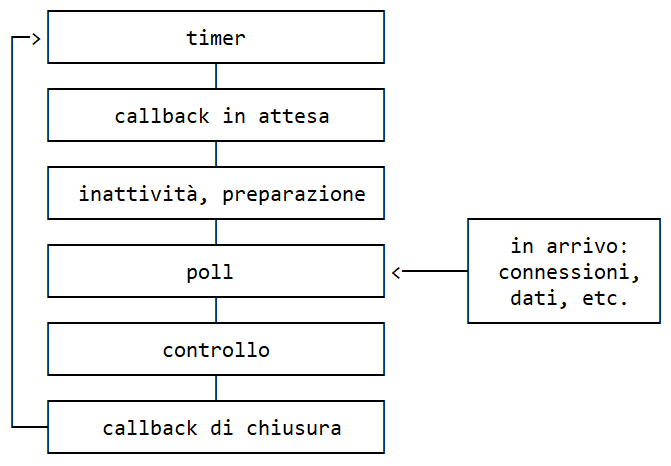
\includegraphics[width=0.8\linewidth]{res/EventLoop.png}
  \caption[Rappresentazione visuale delle transizioni delle fasi dell'event loop.]{Rappresentazione visuale delle transizioni delle fasi dell'event loop.\protect\cite{node.js-eventloop}}
  \label{fig:EventLoop}
\end{center}
\end{figure}

Le fasi dell'event loop sono le seguenti:
\begin{itemize}
\item \textbf{timer}: questa fase esegue le callback programmate da \code{setTimeout()} e \code{setInterval()}.
\item \textbf{callback in attesa}: esegue le callback di input/output prelevate dalla coda di attesa relative a operazioni di sistema, come ad esempio errori TCP.
\item \textbf{inattività, preperazione}: operazioni interne.
\item \textbf{poll}: vengono prelevati e inseriti nella coda nuovi eventi collegati al completamento di operazioni di I/O. Se la coda non è vuota, verranno processate le diverse callback in essa presenti. In caso contrario, se sono state registrate delle callback con la funzione \code{setImmediate()}, verrà terminata questa fase e si passerà alla fase successiva per processarle. Nel caso in cui non siano state registrate callback con la funzione \code{setImmediate()}, l'event loop resta in attesa che vengano aggiunte nuove callback alla coda. Mentre è in questa fase, l'event loop controlla se sono presenti callback che devono essere eseguite nella coda dei timer e, se lo sono, ritorna nella prima fase ed esegue le callback presenti in quella coda.\cite{mrwebmaster}
\item \textbf{controllo}: vengono invocate le callback \code{setImmediate()}.
\item \textbf{callback di chiusura}: vengono gestiti gli eventi di chiusura, per pulire lo stato dell'applicazione.
\end{itemize}

La funzione \code{process.nextTick()} viene eseguita subito dopo il completamento dell'operazione corrente, indipendentemente dalla fase in cui l'event loop si trova. È principalmente utilizzata per gestire errori, risorse non necessarie, ritentare richieste non andate a buon fine, oppure per effettuare operazioni dopo l'esaurimento dello stack delle chiamate ma prima che l'event loop continui.\cite{node.js-eventloop}

\subsection{Npm}
Il package manager \textbf{npm} è una raccolta di pacchetti gratuiti o a pagamento utilizzabili sul proprio progetto di sito web.
Utilizzabile al seguito dell’installazione di Node.js viene messo a disposizione come strumento da linea di comando con il quale scaricare moduli JavaScript poi disponibili all’interno del proprio progetto. Viene data la possibilità allo sviluppatore di caricare i propri moduli per metterli a disposizione della community.

\subsection{Express.js}
\textbf{Express.js} è un framework per applicazioni web Node.js flessibile e leggero che fornisce una serie di funzioni avanzate per applicazioni web e dispositivi mobili.

Permette di gestire le richieste HTTP tramite middleware, funzioni con accesso all’oggetto richiesta \texttt{req}, all’oggetto risposta \texttt{res} e alla successiva funzione middleware nel ciclo richiesta-risposta dell’applicazione.

Quando il server riceve una richiesta HTTP la racchiude all’interno di un oggetto ServerRequest. Questo oggetto, insieme all’oggetto ServerResponse, viene passato al primo middleware che ne può modificare il contenuto o aggiungere proprietà.

\subsection{MongoDB}
\textbf{MongoDB} è un DBMS non relazionale open source che utilizza un modello orientato ai documenti, il quale supporta diverse forme di dati. È una delle numerose tecnologie di database non relazionali nate a metà degli anni 2000 sotto il nome di NoSQL per l'utilizzo in applicazioni per big data e altre operazioni di elaborazione di dati che non beneficiano dell'utilizzo di modelli relazionali rigidi. L'architettura MongoDB è composta da collezioni e documenti, piuttosto che da tabelle e righe.

In MongoDB, un record è un documento, che consiste in una struttura dati composta da coppie di campo e valore. I documenti MongoDB usano una variante degli oggetti JSON chiamata Binary JSON (BSON), che può contenere ulteriori tipologie di dati.
I campi dei documenti sono analoghi alle colonne dei database relazionali, e i valori in essi contenuti possono essere una varietà di tipi di dati, tra cui altri documenti, array e array di documenti.

I documenti, forniti di una chiave primaria come identificatore univoco, sono l'unità di base dei dati in MongoDB. Le collezioni contengono insiemi di documenti, e sono analoghe alle tabelle nei database relazionali. Le collezioni possono contenere qualsiasi tipo di dato, ma come restrizione i dati in una collezione non possono essere sparsi in altri database.

La mongo shell è un'interfaccia JavaScript a MongoDB interattiva che permette di effettuare interrogazioni e aggiornamenti sui dati, oltre ad eseguire operazioni di amministrazione. La shell è un componente standard delle distribuzioni open source di MongoDB. Una volta installato MongoDB, gli utenti connettono la mongo shell alle istanze MongoDB in esecuzione.

Il formato BSON con cui sono conservati i documenti permette di rappresentare i dati in forma binaria; ciò rende possibile lo sharding automatico, una proprietà chiave di MongoDB che permette alle collezioni di essere distribuite su molteplici sistemi a seguito della crescita del volume dei dati da conservare.

A differenza di altri database NoSQL, MongoDB non richiede l'utilizzo di schemi di database (strutture logiche dei dati contenuti nel database) predefiniti e memorizza qualsiasi tipo di dato. Ciò dà agli utenti la flessibilità di creare un qualsiasi numeri di campi in un documento, facilitando la scalabilità dei database MongoDB rispetto a quelli relazionali. 

Il fatto di poter disporre di un oggetto JSON-like permette una rapida manipolazione delle informazioni, senza necessitare di operazioni di join e quindi ridurre il costo delle operazioni.\cite{searchdatamanagement}

\subsection{Mongoose}
\textbf{Mongoose} è una libreria di Object Data Modelling (ODM) per MongoDB e Node.js. Gestisce le relazioni tra i dati, permette la definizione di schemi, ed è utilizzata come convertitore tra oggetti nel codice e la loro rappresentazione in MongoDB.

\begin{figure}[h]
  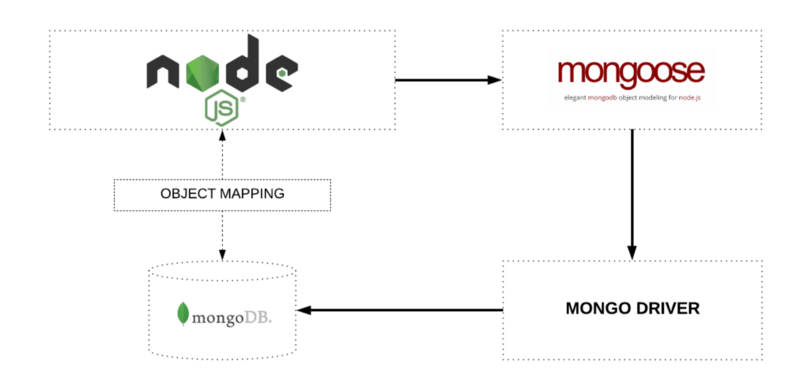
\includegraphics[width=\linewidth]{res/Mongoose.png}
  \caption[Mappatura di oggetti tra Node e MongoDB tramite Mongoose.]{Mappatura di oggetti tra Node e MongoDB tramite Mongoose.\protect\cite{freecodecamp}}
  \label{fig:Mongoose}
\end{figure}

La chiamata \code{require("mongoose")} restituisce un oggetto Singleton, così come avviene per qualsiasi modulo importato in ES6. Ciò significa che alla prima chiamata verrà creata e restituita un'istanza della classe \texttt{Mongoose}, e alle chiamate successive verrà restituita la stessa istanza creata precedentemente e restituita la prima volta.\cite{freecodecamp}

Uno schema descrive il costrutto dei dati di un documento, ovvero definisce il nome e il tipo di ciascun elemento. È ragionevole associare uno schema a ciascuna collezione presente nel database. Un esempio di schema in Mongoose è il seguente:

\begin{lstlisting}
var userSchema = new mongoose.Schema({
 name: String,
 email: String,
 createdOn: Date,
 verified: Boolean
});
\end{lstlisting}

Un altro elemento chiave di Mongoose è il cosiddetto modello. Esso è la versione compilata dello schema; un'istanza del modello verrà mappata a un documento nel database. Si occupa di gestire la lettura, la creazione, l'aggiornamento e la cancellazione dei documenti.\cite{holmes}
\begin{lstlisting}
var User = mongoose.model("User", userSchema);
\end{lstlisting}

Le specifiche di connessione tra Mongoose e il database sono contenute nella cosiddetta stringa di connessione, espressa nel seguente formato:\cite{connection-string}
\begin{lstlisting}
mongodb://[username:password@]host1[:port1][,...hostN[:portN]][/[database][?opzioni]]
\end{lstlisting}

Vi sono due metodi per effettuare la connessione al database con Mongoose: \texttt{mongoose.connect} e \code{createConnection}.\cite{holmes-connection}

Il primo imposta la connessione di default, la quale sarà accessibile da qualsiasi punto dell'applicazione se impostata correttamente.
\begin{lstlisting}
var dbURI = "mongodb://localhost/mydatabase";
mongoose.connect(dbURI);
\end{lstlisting}
Il secondo viene utilizzato nel caso sia necessario stabilire più di una connessione, che sia allo stesso database che a un altro.
\begin{lstlisting}
var dbURI = "mongodb://localhost/myadmindatabase";
var adminConnection = mongoose.createConnection(dbURI);
\end{lstlisting}

\subsection{Textract}
\textbf{Textract} è una libreria Python atta all'estrazione del testo da un file. Supporta l'estrazione da file di diversi formati comuni appoggiandosi a parser dedicati.

Una volta invocato, il metodo \texttt{texttract.process('path/to/file.extension')} instrada il nome del file al parser appropriato e restituisce il testo estratto come stringa di byte codificata con la codifica specificata.\cite{textract}

\subsection{Tesseract}
\textbf{Tesseract} è un motore di riconoscimento ottico dei caratteri OCR sviluppato dalla Hewlett-Packard tra il 1985 e il 1995; è stato abbandonato a se stesso per i successivi 10 anni, fino a quando nel 2005 ne è stato rilasciato il codice
sorgente con una licenza libera. Dal 2006 a novembre 2018 è stato sviluppato da Google.

È considerato uno dei più accurati motori OCR attualmente disponibili, con il vantaggio, non indifferente, che essendo free software è accessibile e utilizzabile da tutti.
Supporta la codifica Unicode (UTF-8), può riconoscere oltre 100 lingue.

Tesseract 4 aggiunge un nuovo motore OCR basato sulla rete neurale (LSTM) che si concentra sul riconoscimento della linea, ma supporta anche il motore OCR Tesseract legacy di Tesseract 3 che funziona riconoscendo i modelli di caratteri.

\subsubsection{Python-tesseract}
\textbf{Python-tesseract} è un wrapper per il motore Tesseract-OCR di Google. È utile come script di invocazione autonomo per tesseract, poiché può leggere tutti i tipi di immagine supportati dalle librerie di immagini Pillow e Leptonica, inclusi jpeg, png, gif, bmp, tiff e altri. Inoltre, se usato come script, Python-tesseract stamperà il testo riconosciuto invece di scriverlo su un file.

\subsection{PDFMiner}
\textbf{PDFMiner} è una libreria per l’analisi di documenti PDF scritta in Python. Oltre al testo, estrae anche le posizioni corrispondenti, i nomi dei caratteri, le dimensioni dei caratteri, la direzione di scrittura (orizzontale o verticale) per ciascun segmento di testo. Non riconosce il testo nelle immagini.

PDFMiner si basa sulla ricostruzione di alcune delle informazioni contenute nel formato PDF, adottando una strategia di parsing lazy, cioè quella di analizzare le istruzioni della struttura del documento PDF solo quando è necessario.
Per effettuare il parsing è necessario utilizzare almeno le classi \texttt{PDFParser}, che si occupa di recuperare i dati dal file, e \texttt{PDFDocument}, che si occupa di memorizzare i dati recuperati.
Per elaborare il contenuto della pagine viene utilizzata la classe \texttt{PDFPageInterpreter}. \texttt{PDFDevice} converte il contenuto in formati diversi. \texttt{PDFResourceManager} viene utilizzato per archiviare risorse condivise come caratteri o immagini.
	\clearpage{\pagestyle{empty}\cleardoublepage}
\chapter{Implementazione}                %crea il capitolo
%%%%%%%%%%%%%%%%%%%%%%%%%%%%%%%%%%%%%%%%%imposta l'intestazione di pagina
\section{Frontend}
Il frontend è stato sviluppato utilizzando Angular 8, utilizzando Angular CLI per installare librerie ed eseguire l'applicazione.

L'applicazione è suddivisa in sottocartelle per ciascun componente:
\begin{itemize}
	\item \texttt{home}: componente il cui contenuto è accessibile solo a seguito dell'autenticazione. Nel caso l'utente autenticato sia uno studente, verrà renderizzato il componente \texttt{dashboard-user}.
	\item \texttt{login}: permette l'accesso dell'utente registrato nel sistema, sarà accessibile a chi non ha eseguito l'accesso.
	\item \texttt{register}: permette la registrazione di un utente. È utilizzato per due route diverse, relative alla registrazione dello studente e alla registrazione del docente, per cui verranno richiesti campi diversi.
	\item \texttt{dashboard-user}: componente attraverso il quale vengono sottomesse al sistema di raccomandazione le diverse richieste per ottenere il learning path utilizzando come dati di input le informazioni associate all'utente autenticato. L'invio delle richieste avviene attraverso tre form corrispondenti all'invio di informazioni per ciascun step della produzione del learning path:
\begin{itemize}
\item \textit{richiesta dei dipartimenti e delle facoltà consigliate}: vengono utilizzate come input le informazioni dello studente associate al momento della registrazione
\item \textit{richiesta dei corsi consigliati}: una volta ottenuti i dipartimenti e le facoltà consigliate, l'utente può inviare la richiesta per visualizzare i corsi consigliati dal sistema di raccomandazione selezionando il dipartimento, la facoltà e l'anno di interesse
\item \textit{richiesta delle risorse consigliate}: una volta selezionato il corso di interesse tra quelli consigliati, verranno visualizzate le risorse suggerite sulla base dei dati dello studente
\end{itemize}
	\item \texttt{profile-teacher}: pannello che permette al docente di associare nuovi corsi al suo profilo tra quelli memorizzati nel sistema
	\item \texttt{dashboard-courses}: vengono visualizzate le informazioni dei corsi. Gli amministratori possono modificarle.
	\item \texttt{dashboard-resources}: pannello visualizzabile in home dai docenti e dagli amministratori, permette il caricamento di nuove risorse didattiche ai corsi di cui sono titolari.
\end{itemize}

La gestione delle richieste al server backend è contenuta nei metodi di servizi dedicati.

\subsection{Servizio di autenticazione}
Il servizio di autenticazione contiene la logica delle funzioni di login, logout e registrazione, utilizzabili dai componenti del sistema.

I subject e gli observable della libreria RxJS sono usati per tenere traccia dell'utente attualmente loggato e notificare del login e del logout, mediante il metodo \texttt{this.currentUserSubject.next()}, i componenti che eseguono \texttt{subscribe()} sull'oggetto \texttt{currentUser}.

Il metodo \texttt{login()} invia al server una richiesta POST per l'autenticazione utilizzando le credenziali dell'utente. Se l'utente è presente nel database, le sue informazioni verranno memorizzate nel local storage per tenere traccia del login in tutte le pagine.

Il metodo \texttt{login()} rimuove dal local storage le informazioni relative all'utente loggato e imposta \texttt{currentUserSubject} a \texttt{null}, notificando i subscriber del logout.

Il metodo \texttt{register()} invia al server una richiesta POST per la registrazione dell'utente, per poi proseguire con la chiamata di \texttt{login()}.

\subsection{Classi di utility}
L'\textbf{Auth Guard} è un Route Guard usato per limitare l'accesso a determinati route a utenti autorizzati, passato come parametro \texttt{canActivate} ai percorsi di route interessati. Il metodo \texttt{canActivate()}, invocato ogni volta che qualcuno tenterà di accedere al route associato, restituisce un valore booleano che indica se consentire o meno la navigazione. Se l’utente non è autenticato, verrà reindirizzato alla route di login.

\vspace{5mm}

L'\textbf{Error Interceptor} intercetta le risposte delle richieste API e provvede a eseguire il logout dall'applicazione in caso di errori. Implementa la classe HttpInterceptor della libreria \texttt{@angular/common} ed è aggiunto tra i provider dell'applicazione. Grazie alle informazioni presenti nell'oggetto Provider, il Root Injector sa come creare e recuperare un'istanza dell'ErrorInterceptor quando serve e fornirla a qualsiasi componente, direttiva o altro servizio che ne faccia richiesta.

\vspace{5mm}

Il \textbf{JWT Interceptor} intercetta le richieste invocate per aggiungere un token JWT di autenticazione nell'header qualora l'utente dovesse essere loggato.

\section{Backend}
Oltre alle richieste eseguite al Pathadora Engine per ottenere il learning path suggerito e aggiungere individual nell'ontologia, viene utilizzato un server Express per gestire l'autenticazione degli utenti e accedere alle proprietà degli oggetti aggiunti memorizzati in un database MongoDB.

Il server viene avviato lanciando il file \texttt{server.js}, attraverso il quale viene creata un'istanza Express, viene stabilita una connessione col database MongoDB e vengono definite le diverse route utilizzate dall'applicazione.

Nello sviluppo è stato utilizzato il tool Robo3T per manipolare gli oggetti nelle collezioni del database. La validità delle richieste è stata testata con Postman.

Le route sono suddivise nei seguenti moduli, ciascuno dei quali fa riferimento a uno schema Mongoose utilizzato nel database:
\begin{itemize}
	\item \texttt{users}
	\begin{itemize}
		\item \texttt{/register} (post): carica nel database un nuovo utente utilizzando le informazioni del corpo dell'oggetto richiesta e effettua il login di quest'ultimo assegnandogli un token. Viene inoltre eseguito l'inserimento di un individual Learner nell'ontologia Pathadora;
		\item \texttt{/} (get): restituisce i dati di tutti gli utenti registrati nel database;
		\item \texttt{/me} (get): restituisce i dati dell'utente loggato;
		\item \texttt{/courses} (get): restituisce i dati dei corsi associati all'utente autenticato, nel caso quest'ultimo abbia il ruolo \texttt{teacher};
		\item \texttt{/courses} (post): riceve come input un array di id di corsi e li associa al docente autenticato;
		\item \texttt{/courses/:id} (delete): rimuove il corso con id specificato dall'elenco dei corsi associati al docente; autenticato
	\end{itemize}
	\item \texttt{auth}
	\begin{itemize}
		\item \texttt{/} (get): restituisce le informazioni relative all'utente loggato
		\item \texttt{/} (post): effettua il login dell'utente con email e password sottomesse generando un token
	\end{itemize}
	\item \texttt{courses}
	\begin{itemize}
		\item \texttt{/} (get): restituisce i dati di tutti i corsi registrati nel database
		\item \texttt{/:id} (get): restituisce le informazioni associate al corso con id specificato
		\item \texttt{/} (post): se l'utente autenticato ha il ruolo \texttt{admin}, registra un nuovo corso. Viene inoltre eseguito l'inserimento di un individual Course nell'ontologia Pathadora.
		\item \texttt{/:id} (post): se l'utente autenticato ha il ruolo \texttt{admin}, aggiorna il corso con id specificato
		\item \texttt{/:id} (delete): se l'utente autenticato ha il ruolo \texttt{admin}, rimuove il corso con id specificato
		\item \texttt{/resource/:course\_id} (post): se l'utente autenticato ha il ruolo \texttt{teacher}, associa una risorsa al corso con id associato. Il file viene caricato utilizzando il middleware Multer di Express, memorizzato in una directory di file statici accessibili mediante richiesta HTTP. Viene inoltre eseguito l'inserimento di un individual LearningObject nell'ontologia Pathadora.
	\end{itemize}
\end{itemize}

Per le route che richiedono la verifica dell'identità dell'utente loggato è utilizzata una funzione middleware che accede al token associato all'header della richiesta, decodificandolo con JWT per ottenere come output le informazioni dell'utente che potranno poi essere utilizzate dall'handler associato alla route.

\section{Estrazione e generazione dei metadati}
Al caricamento di una risorsa associata a un corso, viene invocato un processo Python che calcola una serie di metadati relativi alle proprietà della risorsa e del suo contenuto di cui il modello di profilazione farà uso nel calcolo del suggerimento delle risorse consigliate.

\subsection{Estrazione dei metadati intrinseci del file}
Al caricamento di una risorsa associata a un corso, i metadati a essa associati vengono estratti mediante la libreria \texttt{metadata-extract}, che a sua volta fa uso di diversi estrattori per più estensioni.

\subsection{Grado di leggibilità di Flesh-Kincaid}
Viene inoltre calcolato attraverso uno script Python un metadato relativo al grado di leggibilità del testo contenuto nel file, utilizzando la formula di \textbf{Flesh-Kincaid}. Più il valore è alto, più il testo risulta essere semplice da leggere.

\[ F=206,835-(84,6*S)-(1,015*P) \]

La difficoltà di lettura dipende da S e da P, rispettivamente il numero medio di sillabe contenute in una parola e il numero medio di parole contenute in una frase.

La scelta dei coefficienti è una conseguenza di un processo di affinamento del grado di istruzione di una persona in grado di leggere e comprendere la lingua inglese, ottimizzati in modo che venga restituito un valore compreso tra 0 e 100. Viene data più importanza al valore di S piuttosto che a P.\cite{readibility}

\subsection{Accessibilità delle immagini in un documento}
È stato prodotto uno script Python attraverso cui viene restituito un indicatore di accessibilità del testo contenuto nelle immagini presenti in un documento PDF.

Per ciascuna immagine presente nel documento, estrapolate mediante la libreria Python-tesseract, vengono catturate le aree che contengono testo ed estratto il colore dei caratteri in formato RGB (prelevando il colore più rilevante nella textbox analizzata). Viene poi calcolato il rapporto di contrasto tra questo colore e il colore di sfondo dell'immagine, seguendo i criteri di WCAG 2 dove il range di differenza di luminosità tra i due colori varia da 1 (ad esempio bianco su bianco) a 21 (ad esempio nero su bianco). 

Viene poi calcolata la media dei rapporti relativi alle immagini di ciascun file, e il risultato finale corrisponderà alla media di questi risultati per ogni file.

Il livello minimo per cui il contenuto può essere considerato accessibile è 4.5.

\subsection{Dimensione minima del carattere in un documento}
È stato prodotto uno script Python attraverso cui viene restituito il valore della dimensione minima dei caratteri individuata in un documento PDF. Più è basso il valore meno il contenuto è accessibile agli utenti con problemi visivi.

La scansione delle pagine e del relativo contenuto testuale è eseguita mediante la libreria PDFMiner.
	

	%%%%%%%%%%%%%%%%%%%%%%%%%
	% inizio parte finale del documento
	%
	% eventuali appendici, bibliografia obbligatoria,
	% eventuale lista delle tabelle e delle figure (nel caso decommentare 
	% la riga con i comandi \listoffigures e \listoftables)
	%%%%%%%%%%%%%%%%%%%%%%%%%
	
    %%%%%%%%%%%%%%%%%%%%%%%%%%%%%%%%%%%%%%%%%non numera l'ultima pagina sinistra
\clearpage{\pagestyle{empty}\cleardoublepage}
%%%%%%%%%%%%%%%%%%%%%%%%%%%%%%%%%%%%%%%%%per fare le conclusioni
\chapter*{Conclusioni}
%%%%%%%%%%%%%%%%%%%%%%%%%%%%%%%%%%%%%%%%%imposta l'intestazione di pagina
\rhead[\fancyplain{}{\bfseries
CONCLUSIONI}]{\fancyplain{}{\bfseries\thepage}}
\lhead[\fancyplain{}{\bfseries\thepage}]{\fancyplain{}{\bfseries
CONCLUSIONI}}
%%%%%%%%%%%%%%%%%%%%%%%%%%%%%%%%%%%%%%%%%aggiunge la voce Conclusioni
                                        %   nell'indice
\addcontentsline{toc}{chapter}{Conclusioni}

L'obiettivo di questa tesi è quello di illustrare le tematiche e le fasi di lavoro che hanno interessato lo sviluppo di un sistema di raccomandazione di facoltà, corsi e risorse didattiche e della generazione di metadati che descrivano il contenuto delle risorse didattiche prese a carico.

\vspace{5mm}

Lo sviluppo dell'interfaccia web e delle tecniche di generazione di metadati è stato effettuato in parallelo con lo sviluppo del modello di raccomandazione del percorso accademico e del percorso di apprendimento dello studente, che si basa su regole
che estendono e inferiscono nuove relazioni semantiche tra i componenti dell’ontologia che modella il dominio.

\vspace{5mm}

L'applicazione sviluppata è stata testata su più browser (Google Chrome, Mozilla Firefox, Microsoft Edge), risulta funzionante e restituisce risultati corretti se configurata adeguatamente.

Lo sviluppo di tecniche di generazione automatica di metadati si è focalizzato sulle risorse didattiche di tipo testuale; un possibile approfondimento potrebbe comprendere la generazione di metadati relativi a risorse multimediali, basate sull'estrazione del testo udibile nella sorgente audio come discusso nella capitolo dello stato dell'arte.

    \clearpage{\pagestyle{empty}\cleardoublepage}


\rhead[\fancyplain{}{\bfseries BIBLIOGRAFIA}]{\fancyplain{}{\bfseries\thepage}}
\lhead[\fancyplain{}{\bfseries\thepage}]{\fancyplain{}{\bfseries BIBLIOGRAFIA}}
%%%%%%%%%%%%%%%%%%%%%%%%%%%%%%%%%%%%%%%%% aggiunge l'intestazione di pagina

\addcontentsline{toc}{chapter}{Bibliografia}
%%%%%%%%%%%%%%%%%%%%%%%%%%%%%%%%%%%%%%%%% aggiunge la voce Bibliografia nell'indice





\bibliography{backMatter/biblio}{}



    \rhead[\fancyplain{}{\bfseries \leftmark}]{\fancyplain{}{\bfseries
\thepage}}
%%%%%%%%%%%%%%%%%%%%%%%%%%%%%%%%%%%%%%%%%aggiunge la voce Bibliografia
                                        %   nell'indice
\addcontentsline{toc}{chapter}{Ringraziamenti}

%%%%%%%%%%%%%%%%%%%%%%%%%%%%%%%%%%%%%%%%%non numera l'ultima pagina sinistra
\clearpage{\pagestyle{empty}\cleardoublepage}
\chapter*{Ringraziamenti}
\thispagestyle{empty}
Ringrazio la relatrice Catia Prandi e la correlatrice Chiara Ceccarini per la disponibilità dimostrata e i suggerimenti proposti durante lo svolgimento del lavoro di tesi.

Ringrazio infine tutti coloro che mi hanno sostenuto durante questo percorso universitario e che hanno creduto nel raggiungimento di questo mio importante traguardo.
	
		
	%\input{./Appendice/appendice.tex}
	%\clearpage{\pagestyle{empty}\cleardoublepage}


\rhead[\fancyplain{}{\bfseries BIBLIOGRAFIA}]{\fancyplain{}{\bfseries\thepage}}
\lhead[\fancyplain{}{\bfseries\thepage}]{\fancyplain{}{\bfseries BIBLIOGRAFIA}}
%%%%%%%%%%%%%%%%%%%%%%%%%%%%%%%%%%%%%%%%% aggiunge l'intestazione di pagina

\addcontentsline{toc}{chapter}{Bibliografia}
%%%%%%%%%%%%%%%%%%%%%%%%%%%%%%%%%%%%%%%%% aggiunge la voce Bibliografia nell'indice





\bibliography{backMatter/biblio}{}



	
	\nocite{*}

	%\cleardoublepage
	%\addcontentsline{toc}{chapter}{Bibliografia}


	
	%\listoffigures
	%\listoftables


\end{document}
